\begin{frame}
\frametitle{Example 1: SEND+MORE=MONEY}
\begin{itemize}
\item Example of Finite Domain Constraint Problem
\item Models and Programs
\item Constraint Propagation and Search
\item Some Basic Constraints: linear arithmetic, alldifferent, disequality
\item A Built-in search
\item Visualizers for variables, constraints and search
\end{itemize}
\end{frame}


\section{Problem}
Let's start with the problem.

\begin{frame}<presentation>
\frametitle{Problem Definition}
\begin{block}{A Crypt-Arithmetic Puzzle}
We begin with the definition of the SEND+MORE=MONEY puzzle. It is often shown in the form of a hand-written addition:
\end{block}
\begin{center}
\begin{tabular}{rrrrr}
  & S & E & N & D \\
+ & M & O & R & E \\ \hline
M & O & N & E & Y
\end{tabular}

\end{center}
{\small The puzzle was first proposed by \href{https://en.wikipedia.org/wiki/Henry_Dudeney}{Henry Dudeney} in the \href{https://en.wikipedia.org/wiki/The_Strand_Magazine}{Strand Magazine} from 1924.} 
\end{frame}

\begin{figure}[ht]
\caption{\label{sendmore:problem}Problem Definition}
\begin{center}
\begin{tabular}{rrrrr}
  & S & E & N & D \\
+ & M & O & R & E \\ \hline
M & O & N & E & Y
\end{tabular}

\end{center}
\end{figure}



SEND+MORE=MONEY is a crypt-arithmetic\index{crypt-arithmetic} puzzle, where characters encode numbers and we have to deduce which character stands for which digit. It is one of the classical, early examples of constraint programming, showing how the constraint reasoning mimics the human reasoning when solving this type of problem. The arithmetic problem is usually shown in the form of a handwritten addition. The puzzle is defined by the following rules:


\begin{frame}
\frametitle{Rules}
\only<presentation>{
\begin{textblock}{3.5}(9,6)
\scalebox{0.7}{
\begin{tabular}{rrrrr}
  & S & E & N & D \\
+ & M & O & R & E \\ \hline
M & O & N & E & Y
\end{tabular}

}
\end{textblock}
}
\begin{itemize}
\item Each character stands for a digit from 0 to 9.
\item Numbers are built from digits in the usual, positional notation. 
\item Repeated occurrence of the same character denote the same digit.
\item Different characters denote different digits.
\item Numbers do not start with a zero.
\item The equation must hold.
\end{itemize}
\end{frame}

\lstset{escapechar=@,emph={alldifferent,labeling,::,module,export,lib},emphstyle=\bf,language=Prolog}

\section{Program}

If we want to model this problem as a finite domain constraint problem, we have to define variables and constraints. {\em Variables}\index{variable} range over {\em domains}\index{domain}, which describe the possible values they can take. In this section we consider only finite domains\index{finite domain}, indeed only finite subsets of natural numbers. We will consider constraint problems with non-integral domains in a later chapter. 

An {\em assignment}\index{assignment} is a mapping from the variables to values in their respective domains.

A {\em constraint}\index{constraint} ranges over one or multiple variables and expresses a condition which must hold between these variables. Constraints can take many forms, they may be explicit\index{constraint!explicit}, describing combinations of values that are allowed or excluded, or symbolic\index{constraint!symbolic}, for example in the form of arithmetic constraints\index{constraint!arithmetic}. Formally, we can see a constraint as a subset of the Cartesian product of the domains of its variables. An assignment {\em satisfies} a constraint if its projection on the variables of the constraint belong to this constrained subset.

An assignment of values to variables is a {\em solution}\index{solution} if all constraints are satisfied.

For many problems, we have considerable choices in selecting the variables and constraints. Often, models differ dramatically in the number of variables needed, the complexity and number of constraints used to describe the problem, and the speed by which a constraint solver can find a solution.

\begin{frame}<presentation>
\frametitle{Model}
\begin{itemize}
\item Each character is a variable, which ranges over the values 0 to 9.
\item An {\em alldifferent} constraint between all variables, which states that two different variables must have different values. This is a very common constraint, which we will encounter in many other problems later on.
\item Two {\em disequality constraints} (variable $X$ must be different from value $V$) stating that the variables at the beginning of a number can not take the value 0.
\item An arithmetic {\em equality constraint} linking all variables with the proper coefficients and stating that the equation must hold.
\end{itemize}
\end{frame}

For the small puzzle considered here, the choice of the variables is fairly obvious: Each character is a variable, which ranges over the values 0 to 9.

For the constraints, a natural description would be:
\begin{itemize}
\item An {\em alldifferent}\index{alldifferent} constraint between all variables, which states that two different variables must have different values. This is a very common constraint, which we will encounter in many other problems later on.
\item Two {\em disequality constraints}\index{disequality constraint}\index{constraint!disequality} (variable $X$ must be different from value $V$) stating that the variables at the beginning of a number can not take the value 0.
\item An arithmetic {\em equality constraint}\index{equality constraint}\index{constraint!equality} linking all variables with the proper coefficients and stating that the equation must hold.
\end{itemize}
Remember that this is not the only model of this problem, we will discuss some alternatives later on.

\begin{frame}
\frametitle{SEND+MORE=MONEY Models}
\begin{itemize}
\item ECLiPSe \hyperlink{sendmore:eclipse}{\beamergotobutton{Show}}
\item MiniZinc \hyperlink{sendmore:minizinc}{\beamergotobutton{Show}}
\item NumberJack \hyperlink{sendmore:numberjack}{\beamergotobutton{Show}}
\item CPMpy \hyperlink{sendmore:cpmpy}{\beamergotobutton{Show}}
\item Choco-solver \hyperlink{sendmore:choco}{\beamergotobutton{Show}}
\end{itemize}
\end{frame}

\begin{frame}[fragile]
\frametitle{ECLiPSe Model}
\label{sendmore:eclipse}
\tiny
\begin{verbatim}
:- lib(ic).

sendmore(Digits) :-
    Digits = [S,E,N,D,M,O,R,Y],
    Digits :: [0..9],
    alldifferent(Digits),
    S #\= 0,
    M #\= 0,
                 1000*S + 100*E + 10*N + D
               + 1000*M + 100*O + 10*R + E
    #= 10000*M + 1000*O + 100*N + 10*E + Y,
    labeling(Digits).
\end{verbatim}
\hyperlink{sendmore:continue}{\beamergotobutton{Continue}}
\end{frame}

\begin{frame}[fragile]
\frametitle{MiniZinc Model}
\label{sendmore:minizinc}
\tiny
\begin{verbatim}
include "alldifferent.mzn";
var 0..9: S;
var 0..9: E;
var 0..9: N;
var 0..9: D;
var 0..9: M;
var 0..9: O;
var 0..9: R;
var 0..9: Y;
constraint S != 0;
constraint M != 0;
constraint           1000 * S + 100 * E + 10 * N + D
                   + 1000 * M + 100 * O + 10 * R + E
       = 10000 * M + 1000 * O + 100 * N + 10 * E + Y;
constraint alldifferent([S,E,N,D,M,O,R,Y]);

solve satisfy;
\end{verbatim}
\hyperlink{sendmore:continue}{\beamergotobutton{Continue}}
\end{frame}

\begin{frame}[fragile]
\frametitle{NumberJack Model {\tiny(from \url{https://github.com/eomahony/Numberjack/})}}
\label{sendmore:numberjack}
\tiny
\begin{verbatim}
from Numberjack import *

def get_model():
    model = Model()
    s, m = VarArray(2, 1, 9)  
    e, n, d, o, r, y = VarArray(6, 0, 9)  
    model.add(      s*1000 + e*100 + n*10 + d +
                    m*1000 + o*100 + r*10 + e ==
          m*10000 + o*1000 + n*100 + e*10 + y)
    model.add(AllDiff((s, e, n, d, m, o, r, y)))
    return s, e, n, d, m, o, r, y, model

def solve(param):
    s, e, n, d, m, o, r, y, model = get_model()
    solver = model.load(param['solver'])
    solver.setVerbosity(param['verbose'])
    solver.solve()
\end{verbatim}
\hyperlink{sendmore:continue}{\beamergotobutton{Continue}}
\end{frame}

\begin{frame}[fragile]
\frametitle{CPMpy Model {\tiny(from \url{https://github.com/CPMpy/})}}
\label{sendmore:cpmpy}
\tiny
\begin{verbatim}
from cpmpy import *
import numpy as np

s,e,n,d,m,o,r,y = intvar(0,9, shape=8)
model = Model(
    AllDifferent([s,e,n,d,m,o,r,y]),
    (    sum(   [s,e,n,d] * np.array([       1000, 100, 10, 1]) ) \
       + sum(   [m,o,r,e] * np.array([       1000, 100, 10, 1]) ) \
      == sum( [m,o,n,e,y] * np.array([10000, 1000, 100, 10, 1]) ) ),
    s > 0,
    m > 0,
)

model.solve()
\end{verbatim}
\hyperlink{sendmore:continue}{\beamergotobutton{Continue}}
\end{frame}

\begin{frame}[fragile]
\frametitle{Choco-solver Model {\tiny(from \url{https://choco-solver.org/})}}
\label{sendmore:choco}
\tiny
\begin{verbatim}
Model model = new Model("SEND+MORE=MONEY");
IntVar S = model.intVar("S", 1, 9, false);
IntVar E = model.intVar("E", 0, 9, false);
IntVar N = model.intVar("N", 0, 9, false);
IntVar D = model.intVar("D", 0, 9, false);
IntVar M = model.intVar("M", 1, 9, false);
IntVar O = model.intVar("0", 0, 9, false);
IntVar R = model.intVar("R", 0, 9, false);
IntVar Y = model.intVar("Y", 0, 9, false);

model.allDifferent(new IntVar[]{S, E, N, D, M, O, R, Y}).post();

IntVar[] ALL = new IntVar[]{
    S, E, N, D,
    M, O, R, E,
    M, O, N, E, Y};
int[] COEFFS = new int[]{
    1000, 100, 10, 1,
    1000, 100, 10, 1,
    -10000, -1000, -100, -10, -1};
model.scalar(ALL, COEFFS, "=", 0).post();

Solver solver = model.getSolver();
solver.showStatistics();
solver.showSolutions();
solver.findSolution();
\end{verbatim}
\hyperlink{sendmore:continue}{\beamergotobutton{Continue}}

\end{frame}



Line~\ref{sendmore:module} shows the module declaration. Each file should be a module, and there should be one module per file. All predicates defined in a module are only visible inside the module, unless they are exported.

Line~\ref{sendmore:export} shows an export directive. It states that the predicate \texttt{sendmory} with {\em arity}\index{arity} one (with one argument) should be exported from this module.

Line~\ref{sendmore:ic} contains a library directive\index{directive}\index{library}. We are loading the \texttt{ic} library\index{ic}\index{library!ic}, which defines the {\em I}nterval {\em C}onstraints\index{constraint!interval} in the ECLiPSe language.
 
Lines~\ref{sendmore:predicate}-\ref{sendmore:search} define the \texttt{sendmory} predicate which is the core of our model. It consists of a single clause with the clause head \texttt{sendmory(L)}. The clause has a single argument $L$, which is a list of variables as defined in line~\ref{sendmore:list}. The square brackets denote lists in Prolog.

We next define the domain of the variables in line~\ref{sendmore:domain}. The infix operator \texttt{::}\index{::}\index{domain definition} takes a variable or list of variables as the first (left) argument, and a domain (here \texttt{0..9}) as the second (right) argument.

We then express the \texttt{alldifferent} constraint in line~\ref{sendmore:alldifferent}. This constraint is a built-in constraint in the \texttt{ic} library, and is thus shown in bold.

Lines~\ref{sendmore:disequality}-\ref{sendmore:disequality2} express the two disequality constraints. The \texttt{ic} library defines the operator \verb$#\=$ for this purpose.

The big linear equality constraint is expressed in line~\ref{sendmore:equality}. The operator \texttt{\#=} is used in the \texttt{ic} library.

Finally, we call the builtin search routine \texttt{labeling}\index{labeling} to assign values to the variables.

\begin{frame}
\frametitle{A Note on Syntax}
\label{sendmore:continue}
\begin{itemize}
\item Some formulations may seem simpler than others
\item This largely is an artifact of a very simple problem
\item In most models, you do not write down constraints one by one
\item You create constraints based on data
\item Ease of integration becomes more important than syntax
\item Debugging tools for those who need a debugger :-) 
\end{itemize}
\end{frame}


\begin{frame}
\frametitle{Choice of Model}
\label{sendmore:Choice of model}
\begin{itemize}
\item This is {\em one} model, not {\em the} model of the problem
\item Many possible alternatives
\item Choice often depends on your constraint system
\begin{itemize}
\item Constraints available
\item Reasoning attached to constraints
\end{itemize}
\item Not always clear which is the {\em best} model
\item Often: Not clear what is the {\em problem}
\end{itemize}
\only<presentation>{
%\hyperlink{alternative1}{\beamergotobutton{Alternative 1}}
%\hyperlink{alternative2}{\beamergotobutton{Alternative 2}}
}
\end{frame}

The model we have presented here is {\em one} model of the problem, it is not {\em the} model of the puzzle. Quite often there is a natural way of expressing the problem, but typically there are still many possible alternatives for expressing particular aspects of a model.

The choice which model to use often depends on your constraint system. A system may or may not contain particular constraints, some constraint system have constraint that others don't have and which are difficult to implement in another system. Some constraint systems have special reasoning attached to some constraints, so that they are much more powerful solving some problems than other systems.

Unfortunately, it is not always clear which is the {\em best model}, or if there is indeed a best model for a given problem class. Quite often, we don't even know what exactly the problem is, and we can decide which constraints we want to include and which aspects of a problem we can ignore.

One important aspect of constraint programming is that we want to play with the model, experiment by adding or removing some constraints, to really find out which problem we are going to solve and how we are going to do it.

Indeed, for the puzzle here we have developed two alternative models, which are described at the end of this chapter. There are hyperlinks on the slides to look at these alternatives, or you can use the table of contents of the video to look at them now.


\begin{frame}
  \frametitle{Running the Program (MiniZinc IDE)}
  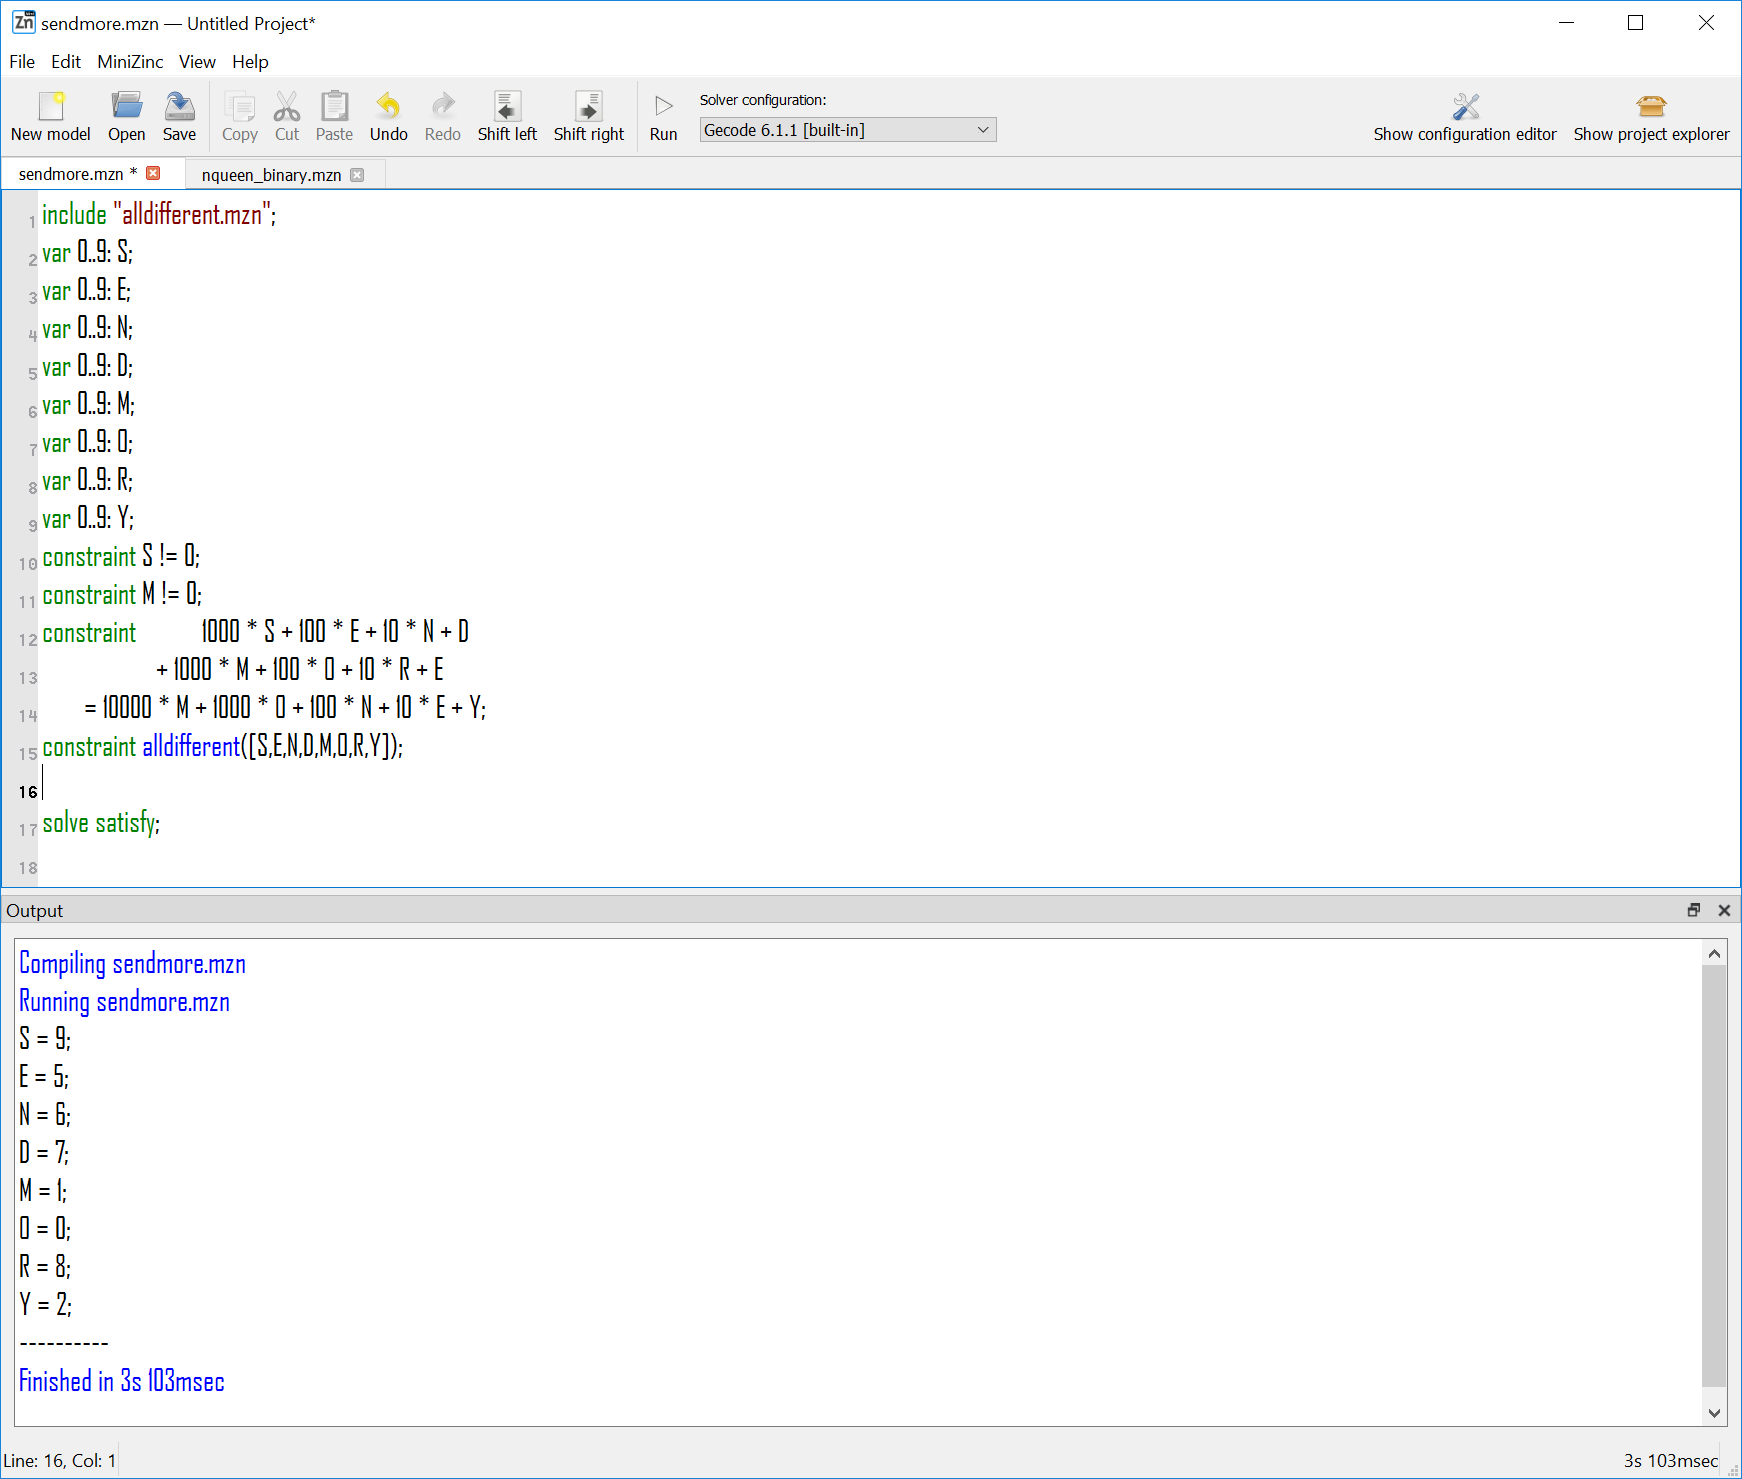
\includegraphics[width=8.5cm]{../sendmore/images/idesendmore}
\end{frame}


If we want to run the program, we have to enter a query \texttt{sendmory:sendmory(L).} which calls the predicate \texttt{sendmory} in the module \texttt{sendmory} with a single argument, a free variable $L$.

The system then returns the answer as a binding for the variable $L$, and it says \texttt{yes}, indicating that it has found a first solution. There may be additional solutions, which can be obtained by backtracking.



\begin{frame}
\frametitle{Question}
\begin{itemize}
\item But how did the program come up with this solution?
  \item We show solution with ECLiPse, other solvers vary slightly
\end{itemize}
\end{frame}

How did the program actually find this solution, what happened in the constraint system before it printed out this message? That is the question we are going to answer in the following sections.

Usually, we are not going to analyze the behaviour of a program in such great detail, but for an introduction I think it is useful to understand how much work can happen inside the constraint engine and how variables, constraints and search interact to find a solution.

\section{Constraint Setup}
We will now go through the constraint setup, where the constraints are created and perform their initial propagation before the search is started. We are going to use different visualization tools to understand what is happening, this gives a much better conceptual model than tracing through the execution with the line debugger.

\subsection{Domain Definition}


\begin{frame}[fragile]
  \frametitle{Domain Definition}
  \begin{semiverbatim}
var 0..9: S;
var 0..9: E;
var 0..9: N;
var 0..9: D;
var 0..9: M;
var 0..9: O;
var 0..9: R;
var 0..9: Y;

  \end{semiverbatim}
\end{frame}

When we first encounter our list of variables, we define them to be domain variables with a domain from 0 to 9.

\begin{frame}<presentation>
\frametitle{Domain Visualization}
\only<2>{
\begin{textblock}{3}(0,5)
Rows = Variables
\end{textblock}
}
\only<3>{
\begin{textblock}{5}(5,0)
Columns = Values
\end{textblock}
}
\only<4>{
\begin{textblock}{3}(5,5)
Cells= State
\end{textblock}
}
\only<1->{
\begin{center}
\begin{tabular}{|c|c|c|c|c|c|c|c|c|c|c|}\hline
  & 0 & 1 & 2 & 3 & 4 & 5 & 6 & 7 & 8 & 9 \\ \hline
S &   &   &   &   &   &   &   &   &   &   \\ \hline
E &   &   &   &   &   &   &   &   &   &   \\ \hline
N &   &   &   &   &   &   &   &   &   &   \\ \hline
D &   &   &   &   &   &   &   &   &   &   \\ \hline
M &   &   &   &   &   &   &   &   &   &   \\ \hline
O &   &   &   &   &   &   &   &   &   &   \\ \hline
R &   &   &   &   &   &   &   &   &   &   \\ \hline
Y &   &   &   &   &   &   &   &   &   &   \\ \hline
\end{tabular}

\end{center}
}
\end{frame}

\begin{figure}[ht]
\caption{\label{sendmore:domainvisualizer}Domain Visualization}
\begin{center}
\begin{tabular}{|c|c|c|c|c|c|c|c|c|c|c|}\hline
  & 0 & 1 & 2 & 3 & 4 & 5 & 6 & 7 & 8 & 9 \\ \hline
S &   &   &   &   &   &   &   &   &   &   \\ \hline
E &   &   &   &   &   &   &   &   &   &   \\ \hline
N &   &   &   &   &   &   &   &   &   &   \\ \hline
D &   &   &   &   &   &   &   &   &   &   \\ \hline
M &   &   &   &   &   &   &   &   &   &   \\ \hline
O &   &   &   &   &   &   &   &   &   &   \\ \hline
R &   &   &   &   &   &   &   &   &   &   \\ \hline
Y &   &   &   &   &   &   &   &   &   &   \\ \hline
\end{tabular}

\end{center}
\end{figure}


We can represent the variables with a {\em domain visualizer}\index{visualizer!domain}\index{domain visualizer} (Figure~\ref{sendmore:domainvisualizer}).
It shows the state of the domain variables at this point. Each line shows one variable, each column one value. Initially, all values are allowed for all variables, this is indicated by white cells.
 

\subsection{Alldifferent Constraint}

\begin{frame}[fragile]
\frametitle{Alldifferent Constraint}
\begin{semiverbatim}
include "alldifferent.mzn";

constraint alldifferent([S,E,N,D,M,O,R,Y]);
\end{semiverbatim}
\begin{itemize}
\item Built-in alldifferent predicate included
\item No initial propagation possible
\item {\em Suspends}, waits until variables are changed
\item When variable is fixed, remove value from domain of other variables
\item {\em Forward checking}
\end{itemize}
\end{frame}

\begin{frame}<presentation>
\frametitle{Alldifferent Visualization}
Uses the same representation as the domain visualizer
\begin{center}
\begin{tabular}{|c|c|c|c|c|c|c|c|c|c|c|}\hline
  & 0 & 1 & 2 & 3 & 4 & 5 & 6 & 7 & 8 & 9 \\ \hline
S &   &   &   &   &   &   &   &   &   &   \\ \hline
E &   &   &   &   &   &   &   &   &   &   \\ \hline
N &   &   &   &   &   &   &   &   &   &   \\ \hline
D &   &   &   &   &   &   &   &   &   &   \\ \hline
M &   &   &   &   &   &   &   &   &   &   \\ \hline
O &   &   &   &   &   &   &   &   &   &   \\ \hline
R &   &   &   &   &   &   &   &   &   &   \\ \hline
Y &   &   &   &   &   &   &   &   &   &   \\ \hline
\end{tabular}

\end{center}
\end{frame}


\subsection{Disequality Constraints}


\begin{frame}<presentation>[fragile]
\frametitle{Disequality Constraints}
\begin{semiverbatim}
constraint S != 0;
constraint M != 0;
\end{semiverbatim}
Remove value from domain
\[
S \in \{1..9\}, M \in \{1..9\}
\]
Constraints solved, can be removed 
\end{frame}


\begin{frame}<presentation>
\frametitle{Domains after Disequality}
\begin{center}
\begin{tabular}{|c|c|c|c|c|c|c|c|c|c|c|}\hline
  & 0 & 1 & 2 & 3 & 4 & 5 & 6 & 7 & 8 & 9 \\ \hline
S &\G &   &   &   &   &   &   &   &   &   \\ \hline
E &   &   &   &   &   &   &   &   &   &   \\ \hline
N &   &   &   &   &   &   &   &   &   &   \\ \hline
D &   &   &   &   &   &   &   &   &   &   \\ \hline
M &\G &   &   &   &   &   &   &   &   &   \\ \hline
O &   &   &   &   &   &   &   &   &   &   \\ \hline
R &   &   &   &   &   &   &   &   &   &   \\ \hline
Y &   &   &   &   &   &   &   &   &   &   \\ \hline
\end{tabular}

\end{center}
\end{frame}


\subsection{Equality Constraint}


\begin{frame}<presentation>
\frametitle{Equality Constraint}
\begin{itemize}
\item Normalization of linear terms
\begin{itemize}
\item Single occurence of variable
\item Positive coefficients
\end{itemize}
\item Propagation
\end{itemize}
\end{frame}


\begin{frame}<presentation>
\frametitle{Normalization}
\only<beamer>{
\only<1>{
\begin{tabular}{rrrrr}
& 1000*S+ & 100*E+ & 10*N+ & D \\
& +1000*M+ & 100*O+ & 10*R+ & E \\ \hline
10000*M+ & 1000*O+ & 100*N+ & 10*E+ & Y
\end{tabular}
}

\only<2>{
\begin{tabular}{rrrrr}
& 1000*S+ & 100*E+ & 10*N+ & D \\
& +{\bf 1000*M}+ & 100*O+ & 10*R+ & E \\ \hline
{\bf 10000*M}+ & 1000*O+ & 100*N+ & 10*E+ & Y
\end{tabular}
}

\only<3>{
\begin{tabular}{rrrrr}
& 1000*S+ & 100*E+ & 10*N+ & D \\
& + & 100*O+ & 10*R+ & E \\ \hline
{\bf 9000*M}+ & 1000*O+ & 100*N+ & 10*E+ & Y
\end{tabular}
}

\only<4>{
\begin{tabular}{rrrrr}
& 1000*S+ & 100*E+ & 10*N+ & D \\
& + & {\bf 100*O}+ & 10*R+ & E \\ \hline
9000*M+ & {\bf 1000*O}+ & 100*N+ & 10*E+ & Y
\end{tabular}
}

\only<5>{
\begin{tabular}{rrrrr}
& 1000*S+ & 100*E+ & 10*N+ & D \\
&  & + & 10*R+ & E \\ \hline
9000*M+ & {\bf 900*O}+ & 100*N+ & 10*E+ & Y
\end{tabular}
}

\only<6>{
\begin{tabular}{rrrrr}
& 1000*S+ & 100*E+ & {\bf 10*N}+ & D \\
&  & + & 10*R+ & E \\ \hline
9000*M+ & 900*O+ & {\bf 100*N}+ & 10*E+ & Y
\end{tabular}
}

\only<7>{
\begin{tabular}{rrrrr}
& 1000*S+ & 100*E+ &  & D \\
&  & + & 10*R+ & E \\ \hline
9000*M+ & 900*O+ & {\bf 90*N}+ & 10*E+ & Y
\end{tabular}
}

\only<8>{
\begin{tabular}{rrrrr}
& 1000*S+ & {\bf 100*E}+ &  & D \\
&  & + & 10*R+ & {\bf E} \\ \hline
9000*M+ & 900*O+ & 90*N+ & {\bf 10*E}+ & Y
\end{tabular}
}

\only<9>{
\begin{tabular}{rrrrr}
& 1000*S+ & 91*E+ &  & D \\
&  & + & 10*R &  \\ \hline
9000*M+ & 900*O+ & 90*N+ &  & Y
\end{tabular}
}
}
\only<handout>{
\begin{tabular}{rrrrr}
& 1000*S+ & 100*E+ & 10*N+ & D \\
& +1000*M+ & 100*O+ & 10*R+ & E \\ \hline
10000*M+ & 1000*O+ & 100*N+ & 10*E+ & Y
\end{tabular}

is transformed into 

\begin{tabular}{rrrrr}
& 1000*S+ & 91*E+ &  & D \\
&  & + & 10*R &  \\ \hline
9000*M+ & 900*O+ & 90*N+ &  & Y
\end{tabular}
}
\end{frame}

\begin{tabular}{rrrrr}
& 1000*S+ & 100*E+ & 10*N+ & D \\
& +1000*M+ & 100*O+ & 10*R+ & E \\ \hline
10000*M+ & 1000*O+ & 100*N+ & 10*E+ & Y
\end{tabular}

is transformed into 

\begin{tabular}{rrrrr}
& 1000*S+ & 91*E+ &  & D \\
&  & + & 10*R &  \\ \hline
9000*M+ & 900*O+ & 90*N+ &  & Y
\end{tabular}

\begin{frame}
\frametitle{Simplified Equation}
\[
1000*S + 91*E + 10*R + D = 9000*M + 900*O+ 90*N + Y
\]
\end{frame}

We now look at the initial propagation of the equality constraint, while noting that the \texttt{alldifferent} constraint is suspended, but will be woken when variables are fixed to values.


\begin{frame}
\frametitle{Propagation}
\only<article>{
We consider the two sides of the equation, taking the domains of the variables into account.
}
\only<beamer| article>{
\only<1>{
\begin{eqnarray*}
\lefteqn{1000*S^{1..9} + 91*E^{0..9} + 10*R^{0..9} + D^{0..9}  =}\\ 
& & 9000*M^{1..9} + 900*O^{0..9}+ 90*N^{0..9} + Y^{0..9} 
\end{eqnarray*}
}
\only<article>{
The left hand side ranges from 1000 to 9918, the right hand side from 9000 to 89919.}
\only<2>{
\begin{eqnarray*}
\lefteqn{\underbrace{1000*S^{1..9} + 91*E^{0..9} + 10*R^{0..9} + D^{0..9}}_{1000..9918} =} \\
 & & \underbrace{9000*M^{1..9} + 900*O^{0..9}+ 90*N^{0..9} + Y^{0..9}}_{9000..89919}
\end{eqnarray*}
}
\only<article>{
If the equation holds, then both sides must be equal. We can therefore consider the intersection of the ranges for left and right hand side.}
\only<3->{
\begin{eqnarray*}
\lefteqn{\underbrace{1000*S^{1..9} + 91*E^{0..9} + 10*R^{0..9} + D^{0..9}}_{9000..9918} =}\\
& & \underbrace{9000*M^{1..9} + 900*O^{0..9}+ 90*N^{0..9} + Y^{0..9}}_{9000..9918}
\end{eqnarray*}
}
}
\only<handout>{
\begin{eqnarray*}
\lefteqn{\underbrace{1000*S^{1..9} + 91*E^{0..9} + 10*R^{0..9} + D^{0..9}}_{1000..9918} =} \\
 & & \underbrace{9000*M^{1..9} + 900*O^{0..9}+ 90*N^{0..9} + Y^{0..9}}_{9000..89919}
\end{eqnarray*}
}
\only<article>{
From this we can deduce the following domain restrictions:

}
\only<4->{
Deduction:
\[
M = 1, S = 9, O \in \{0..1\}
\]
}
\only<presentation>{
\only<5>{
\alert<5>{Why?}\hyperlink{sendmore:Propagation of equality: Result}{\beamergotobutton{Skip}}
}
}
\end{frame}

\begin{frame}
\frametitle{Consider lower bound for $S$}
\only<presentation>{
\begin{textblock}{12}(1,-1)
\scalebox{0.7}{$
\underbrace{1000*S^{1..9} + 91*E^{0..9} + 10*R^{0..9} + D^{0..9}}_{9000..9918} = \underbrace{9000*M^{1..9} + 900*O^{0..9}+ 90*N^{0..9} + Y^{0..9}}_{9000..9918}$}
\end{textblock}
}
\begin{itemize}
\item Lower bound of equation is 9000
\item Rest of lhs (left hand side) $(91*E^{0..9}+10*R^{0..9}+D^{0..9})$ is atmost 918
\item $S$ must be greater or equal to $\frac{9000-918}{1000}=8.082$
\begin{itemize}
\item otherwise lower bound of equation not reached by lhs
\end{itemize}
\item $S$ is integer, therefore $S \geq \lceil \frac{9000-918}{1000} \rceil = 9$
\item $S$ has upper bound of 9, so $S = 9$
\end{itemize}
\end{frame}

\begin{frame}
\frametitle{Consider upper bound of $M$}
\only<presentation>{
\begin{textblock}{12}(1,-1)
\scalebox{0.7}{$
\underbrace{1000*S^{1..9} + 91*E^{0..9} + 10*R^{0..9} + D^{0..9}}_{9000..9918} = \underbrace{9000*M^{1..9} + 900*O^{0..9}+ 90*N^{0..9} + Y^{0..9}}_{9000..9918}$}
\end{textblock}
}
\begin{itemize}
\item Upper bound of equation is 9918
\item Rest of rhs (right hand side) $900*O^{0..9}+ 90*N^{0..9} + Y^{0..9}$ is at least 0
\item $M$ must be smaller or equal to $\frac{9918-0}{9000}=1.102$
\item $M$ must be integer, therefore $M \leq \lfloor \frac{9918-0}{9000} \rfloor = 1$ 
\item $M$ has lower bound of 1, so $M=1$ 
\end{itemize}
\end{frame}

\begin{frame}
\frametitle{Consider upper bound of $O$}
\only<presentation>{
\begin{textblock}{12}(1,-1)
\scalebox{0.7}{$
\underbrace{1000*S^{1..9} + 91*E^{0..9} + 10*R^{0..9} + D^{0..9}}_{9000..9918} = \underbrace{9000*M^{1..9} + 900*O^{0..9}+ 90*N^{0..9} + Y^{0..9}}_{9000..9918}$}
\end{textblock}
}
\begin{itemize}
\item Upper bound of equation is 9918
\item Rest of rhs (right hand side) $9000*1+ 90*N^{0..9} + Y^{0..9}$ is at least 9000
\item $O$ must be smaller or equal to $\frac{9918-9000}{900}=1.02$
\item $O$ must be integer, therefore $O \leq \lfloor \frac{9918-9000}{900} \rfloor = 1$ 
\item $O$ has lower bound of 0, so $O \in \{0..1\}$ 
\end{itemize}
\end{frame}

\begin{frame}<presentation>
\frametitle{Propagation of equality: Result}
\label{sendmore:Propagation of equality: Result}
\begin{center}
\begin{tabular}{|c|c|c|c|c|c|c|c|c|c|c|}\hline
  & 0 & 1 & 2 & 3 & 4 & 5 & 6 & 7 & 8 & 9 \\ \hline
S &\G &\X &\X &\X &\X &\X &\X &\X &\X &\F \\ \hline
E &   &   &   &   &   &   &   &   &   &   \\ \hline
N &   &   &   &   &   &   &   &   &   &   \\ \hline
D &   &   &   &   &   &   &   &   &   &   \\ \hline
M &\G &\F &\X &\X &\X &\X &\X &\X &\X &\X \\ \hline
O &   &   &\R &\R &\R &\R &\R &\R &\R &\R \\ \hline
R &   &   &   &   &   &   &   &   &   &   \\ \hline
Y &   &   &   &   &   &   &   &   &   &   \\ \hline
\end{tabular}

\end{center}
\end{frame}

\begin{figure}[ht]
\caption{\label{sendmore:equalitysetup}Propagation of equality: Result}
\begin{center}
\begin{tabular}{|c|c|c|c|c|c|c|c|c|c|c|}\hline
  & 0 & 1 & 2 & 3 & 4 & 5 & 6 & 7 & 8 & 9 \\ \hline
S &\G &\X &\X &\X &\X &\X &\X &\X &\X &\F \\ \hline
E &   &   &   &   &   &   &   &   &   &   \\ \hline
N &   &   &   &   &   &   &   &   &   &   \\ \hline
D &   &   &   &   &   &   &   &   &   &   \\ \hline
M &\G &\F &\X &\X &\X &\X &\X &\X &\X &\X \\ \hline
O &   &   &\R &\R &\R &\R &\R &\R &\R &\R \\ \hline
R &   &   &   &   &   &   &   &   &   &   \\ \hline
Y &   &   &   &   &   &   &   &   &   &   \\ \hline
\end{tabular}

\end{center}
\end{figure}


So after the initial reasoning of the equality constraint (Figure~\ref{sendmore:equalitysetup}), we have deduced that two variables ($S$ and $M$) must have fixed values and that another variable $O$ can only range between 0 and 1.

\begin{frame}<presentation>
\frametitle{Propagation of alldifferent}
\begin{center}
\only<beamer>{
\only<1>{
\begin{tabular}{|c|c|c|c|c|c|c|c|c|c|c|}\hline
  & 0 & 1 & 2 & 3 & 4 & 5 & 6 & 7 & 8 & 9 \\ \hline
S &\G &\X &\X &\X &\X &\X &\X &\X &\X &\F \\ \hline
E &   &   &   &   &   &   &   &   &   &   \\ \hline
N &   &   &   &   &   &   &   &   &   &   \\ \hline
D &   &   &   &   &   &   &   &   &   &   \\ \hline
M &\G &\F &\X &\X &\X &\X &\X &\X &\X &\X \\ \hline
O &   &   &\R &\R &\R &\R &\R &\R &\R &\R \\ \hline
R &   &   &   &   &   &   &   &   &   &   \\ \hline
Y &   &   &   &   &   &   &   &   &   &   \\ \hline
\end{tabular}
}
\only<2>{
\begin{tabular}{|c|c|c|c|c|c|c|c|c|c|c|}\hline
  & 0 & 1 & 2 & 3 & 4 & 5 & 6 & 7 & 8 & 9 \\ \hline
S &\G &\G &\G &\G &\G &\G &\G &\G &\G &\F \\ \hline
E &   &   &   &   &   &   &   &   &   &\D \\ \hline
N &   &   &   &   &   &   &   &   &   &\D \\ \hline
D &   &   &   &   &   &   &   &   &   &\D \\ \hline
M &\G &\F &\G &\G &\G &\G &\G &\G &\G &\G \\ \hline
O &   &   &\G &\G &\G &\G &\G &\G &\G &\G \\ \hline
R &   &   &   &   &   &   &   &   &   &\D \\ \hline
Y &   &   &   &   &   &   &   &   &   &\D \\ \hline
\end{tabular}
}
\only<3>{
\begin{tabular}{|c|c|c|c|c|c|c|c|c|c|c|}\hline
  & 0 & 1 & 2 & 3 & 4 & 5 & 6 & 7 & 8 & 9 \\ \hline
S &\G &\G &\G &\G &\G &\G &\G &\G &\G &\A \\ \hline
E &   &\D &   &   &   &   &   &   &   &\G \\ \hline
N &   &\D &   &   &   &   &   &   &   &\G \\ \hline
D &   &\D &   &   &   &   &   &   &   &\G \\ \hline
M &\G &\F &\G &\G &\G &\G &\G &\G &\G &\G \\ \hline
O &   &\D &\G &\G &\G &\G &\G &\G &\G &\G \\ \hline
R &   &\D &   &   &   &   &   &   &   &\G \\ \hline
Y &   &\D &   &   &   &   &   &   &   &\G \\ \hline
\end{tabular}
}
\only<4>{
\begin{tabular}{|c|c|c|c|c|c|c|c|c|c|c|}\hline
  & 0 & 1 & 2 & 3 & 4 & 5 & 6 & 7 & 8 & 9 \\ \hline
S &\G &\G &\G &\G &\G &\G &\G &\G &\G &\A \\ \hline
E &   &\G &   &   &   &   &   &   &   &\G \\ \hline
N &   &\G &   &   &   &   &   &   &   &\G \\ \hline
D &   &\G &   &   &   &   &   &   &   &\G \\ \hline
M &\G &\A &\G &\G &\G &\G &\G &\G &\G &\G \\ \hline
O &\F &\G &\G &\G &\G &\G &\G &\G &\G &\G \\ \hline
R &   &\G &   &   &   &   &   &   &   &\G \\ \hline
Y &   &\G &   &   &   &   &   &   &   &\G \\ \hline
\end{tabular}
}
\only<5>{
\begin{tabular}{|c|c|c|c|c|c|c|c|c|c|c|}\hline
  & 0 & 1 & 2 & 3 & 4 & 5 & 6 & 7 & 8 & 9 \\ \hline
S &\G &\G &\G &\G &\G &\G &\G &\G &\G &\A \\ \hline
E &\D &\G &   &   &   &   &   &   &   &\G \\ \hline
N &\D &\G &   &   &   &   &   &   &   &\G \\ \hline
D &\D &\G &   &   &   &   &   &   &   &\G \\ \hline
M &\G &\A &\G &\G &\G &\G &\G &\G &\G &\G \\ \hline
O &\F &\G &\G &\G &\G &\G &\G &\G &\G &\G \\ \hline
R &\D &\G &   &   &   &   &   &   &   &\G \\ \hline
Y &\D &\G &   &   &   &   &   &   &   &\G \\ \hline
\end{tabular}
}
}
\only<6>{
\begin{tabular}{|c|c|c|c|c|c|c|c|c|c|c|}\hline
  & 0 & 1 & 2 & 3 & 4 & 5 & 6 & 7 & 8 & 9 \\ \hline
S &\G &\G &\G &\G &\G &\G &\G &\G &\G &\A \\ \hline
E &\G &\G &   &   &   &   &   &   &   &\G \\ \hline
N &\G &\G &   &   &   &   &   &   &   &\G \\ \hline
D &\G &\G &   &   &   &   &   &   &   &\G \\ \hline
M &\G &\A &\G &\G &\G &\G &\G &\G &\G &\G \\ \hline
O &\A &\G &\G &\G &\G &\G &\G &\G &\G &\G \\ \hline
R &\G &\G &   &   &   &   &   &   &   &\G \\ \hline
Y &\G &\G &   &   &   &   &   &   &   &\G \\ \hline
\end{tabular}

}
\end{center}
\only<6>{
\[
O = 0, [E,R,D,N,Y] \in \{2..8\}
\]
}
\end{frame}

\begin{figure}[ht]
\caption{\label{sendmore:alldifferentprop1}Propagation of \texttt{alldifferent}}
\begin{center}
\begin{tabular}{|c|c|c|c|c|c|c|c|c|c|c|}\hline
  & 0 & 1 & 2 & 3 & 4 & 5 & 6 & 7 & 8 & 9 \\ \hline
S &\G &\G &\G &\G &\G &\G &\G &\G &\G &\A \\ \hline
E &\G &\G &   &   &   &   &   &   &   &\G \\ \hline
N &\G &\G &   &   &   &   &   &   &   &\G \\ \hline
D &\G &\G &   &   &   &   &   &   &   &\G \\ \hline
M &\G &\A &\G &\G &\G &\G &\G &\G &\G &\G \\ \hline
O &\A &\G &\G &\G &\G &\G &\G &\G &\G &\G \\ \hline
R &\G &\G &   &   &   &   &   &   &   &\G \\ \hline
Y &\G &\G &   &   &   &   &   &   &   &\G \\ \hline
\end{tabular}

\end{center}
\end{figure}


The assignment of the variables will wake up the \texttt{alldifferent} constraint. This removes the assigned values 1 and 9 from the domain of the unassigned variables. But variable $O$ could only take values 0 or 1. If we remove value 1, then it must take value 0. This assignment will be propagated through the \texttt{alldifferent} constraint and removes the value 0 from the remaining variables (Figure~\ref{sendmore:alldifferentprop1}.

At this point the equality constraint will be checked again, since some variable bounds have been updated.

\begin{frame}<presentation>
\frametitle{Waking the equality constraint}
\begin{itemize}
\item Triggered by assignment of variables
\item {\em or} update of lower or upper bound 
\end{itemize}
\end{frame}

For ease of presentation, we first remove the constant parts of the constraint, and obtain a simplified form:
\begin{frame}
\frametitle{Removal of constants}
\only<1>{
\begin{eqnarray*}
\lefteqn{1000*9 + 91*E^{2..8} + 10*R^{2..8} + D^{2..8} =} \\
& &  9000*1 + 900*0+ 90*N^{2..8} + Y^{2..8}
\end{eqnarray*}
}
\only<2>{
\begin{eqnarray*}
\lefteqn{{\bf 1000*9} + 91*E^{2..8} + 10*R^{2..8} + D^{2..8} =} \\
& &  {\bf 9000*1} + {\bf 900*0}+ 90*N^{2..8} + Y^{2..8}
\end{eqnarray*}
}
\only<3>{
\[
91*E^{2..8}+10*R^{2..8}+D^{2..8} = 90*N^{2..8}+Y^{2..8}
\]
}
\end{frame}

We now go though several steps of updating variable bounds, each triggering a renewed check of the equality constraint.

\begin{frame}
\frametitle{Propagation of equality (Iteration 1)}
\only<1>{
\[
\underbrace{91*E^{2..8}+10*R^{2..8}+D^{2..8}}_{204..816} = \underbrace{90*N^{2..8}+Y^{2..8}}_{182..728}
\]
}
\only<2->{
\[
\underbrace{91*E^{2..8}+10*R^{2..8}+D^{2..8} = 90*N^{2..8}+Y^{2..8}}_{204..728}
\]
}
\only<3>{
\[
N \geq 3 = \lceil \frac{204-8}{90}\rceil, E \leq 7 = \lfloor \frac{728-22}{91} \rfloor
\]
}
\end{frame}

\begin{frame}
\frametitle{Propagation of equality (Iteration 2)}
\only<1>{
\[
91*E^{2..7}+10*R^{2..8}+D^{2..8} = 90*N^{3..8}+Y^{2..8}
\]
}
\only<2>{
\[
\underbrace{91*E^{2..7}+10*R^{2..8}+D^{2..8}}_{204..725} = \underbrace{90*N^{3..8}+Y^{2..8}}_{272..728}
\]
}
\only<3->{
\[
\underbrace{91*E^{2..7}+10*R^{2..8}+D^{2..8} = 90*N^{3..8}+Y^{2..8}}_{272..725}
\]
}
\only<4>{
\[
E \geq 3 = \lceil \frac{272-88}{91} \rceil
\]
}
\end{frame}



\begin{frame}
\frametitle{Propagation of equality (Iteration 3)}
\only<1>{

\[
91*E^{3..7}+10*R^{2..8}+D^{2..8} = 90*N^{3..8}+Y^{2..8}
\]
}
\only<2>{
\[
\underbrace{91*E^{3..7}+10*R^{2..8}+D^{2..8}}_{295..725} = \underbrace{90*N^{3..8}+Y^{2..8}}_{272..728}
\]
}
\only<3->{
\[
\underbrace{91*E^{3..7}+10*R^{2..8}+D^{2..8} = 90*N^{3..8}+Y^{2..8}}_{295..725}
\]
}
\only<4>{
\[
N \geq 4 = \lceil \frac{295-8}{90} \rceil
\]
}
\end{frame}
\begin{frame}
\frametitle{Propagation of equality (Iteration 4)}
\only<1>{


\[
91*E^{3..7}+10*R^{2..8}+D^{2..8} = 90*N^{4..8}+Y^{2..8}
\]
}
\only<2>{
\[
\underbrace{91*E^{3..7}+10*R^{2..8}+D^{2..8}}_{295..725} = \underbrace{90*N^{4..8}+Y^{2..8}}_{362..728}
\]
}
\only<3->{
\[
\underbrace{91*E^{3..7}+10*R^{2..8}+D^{2..8} = 90*N^{4..8}+Y^{2..8}}_{362..725}
\]
}
\only<4>{
\[
E \geq 4 = \lceil \frac{362-88}{91} \rceil
\]
}
\end{frame}

\begin{frame}
\frametitle{Propagation of equality (Iteration 5)}
\only<1>{
\[
91*E^{4..7}+10*R^{2..8}+D^{2..8} = 90*N^{4..8}+Y^{2..8}
\]
}
\only<2>{
\[
\underbrace{91*E^{4..7}+10*R^{2..8}+D^{2..8}}_{386..725} = \underbrace{90*N^{4..8}+Y^{2..8}}_{362..728}
\]
}
\only<3->{
\[
\underbrace{91*E^{4..7}+10*R^{2..8}+D^{2..8} = 90*N^{4..8}+Y^{2..8}}_{386..725}
\]
}
\only<4>{
\[
N \geq 5 = \lceil \frac{386-8}{90} \rceil
\]
}
\end{frame}

\begin{frame}
\frametitle{Propagation of equality (Iteration 6)}
\only<1>{
\[
91*E^{4..7}+10*R^{2..8}+D^{2..8} = 90*N^{5..8}+Y^{2..8}
\]
}
\only<2>{
\[
\underbrace{91*E^{4..7}+10*R^{2..8}+D^{2..8}}_{386..725} = \underbrace{90*N^{5..8}+Y^{2..8}}_{452..728}
\]
}
\only<3->{
\[
\underbrace{91*E^{4..7}+10*R^{2..8}+D^{2..8} = 90*N^{5..8}+Y^{2..8}}_{452..725}
\]
}
\only<4>{
\[
N \geq 5 = \lceil \frac{452-8}{90} \rceil, E \geq 4 = \lceil \frac{452-88}{91} \rceil
\]
\alert<4>{No further propagation at this point}
}
\end{frame}
We have reached a fixed-point of the constraint propagation, all constraints have been checked, and no further domain reduction is possible.

\begin{frame}<presentation>
\frametitle{Domains after setup}
\begin{center}
\begin{tabular}{|c|c|c|c|c|c|c|c|c|c|c|}\hline
  & 0 & 1 & 2 & 3 & 4 & 5 & 6 & 7 & 8 & 9 \\ \hline
S &\G &\G &\G &\G &\G &\G &\G &\G &\G &\A \\ \hline
E &\G &\G &\G &\G &   &   &   &   &\G &\G \\ \hline
N &\G &\G &\G &\G &\G &   &   &   &   &\G \\ \hline
D &\G &\G &   &   &   &   &   &   &   &\G \\ \hline
M &\G &\A &\G &\G &\G &\G &\G &\G &\G &\G \\ \hline
O &\A &\G &\G &\G &\G &\G &\G &\G &\G &\G \\ \hline
R &\G &\G &   &   &   &   &   &   &   &\G \\ \hline
Y & \G&\G &   &   &   &   &   &   &   &\G \\ \hline
\end{tabular}

\end{center}
\end{frame}

\begin{figure}[ht]
\caption{\label{sendmore:aftersetup}Domains after setup}
\begin{center}
\begin{tabular}{|c|c|c|c|c|c|c|c|c|c|c|}\hline
  & 0 & 1 & 2 & 3 & 4 & 5 & 6 & 7 & 8 & 9 \\ \hline
S &\G &\G &\G &\G &\G &\G &\G &\G &\G &\A \\ \hline
E &\G &\G &\G &\G &   &   &   &   &\G &\G \\ \hline
N &\G &\G &\G &\G &\G &   &   &   &   &\G \\ \hline
D &\G &\G &   &   &   &   &   &   &   &\G \\ \hline
M &\G &\A &\G &\G &\G &\G &\G &\G &\G &\G \\ \hline
O &\A &\G &\G &\G &\G &\G &\G &\G &\G &\G \\ \hline
R &\G &\G &   &   &   &   &   &   &   &\G \\ \hline
Y & \G&\G &   &   &   &   &   &   &   &\G \\ \hline
\end{tabular}

\end{center}
\end{figure}


Figure~\ref{sendmore:aftersetup} shows the state of the variables after the constraint setup, three variables have been assigned, and the domains of the unassigned variables have been reduced.

\clearpage
\section{Search}

We now call the \texttt{labeling}\index{labeling}\index{search} routine to assign values to the unassigned variables.

\begin{frame}<presentation>[fragile]
\frametitle{Search}
solve satisfy;
\begin{itemize}
\item Try to find a feasible solution, choice left to solver
  \item Naive search strategy shown here
\begin{itemize}  
\item Try variable in order given
\item Try values starting from smallest value in domain
\item When failing, backtrack to last open choice
\item {\em Chronological Backtracking}
\item {\em Depth First search}
\end{itemize}
\end{itemize}
\end{frame}

The predicate call
\texttt{labeling([S,E,N,D,M,O,R,Y])}
in line~\ref{sendmore:search} on page~\pageref{sendmore:search} will enumerate the variables in the given order, each time starting with the smallest value in the domain. If the assignment of that value fails, the next value will be tried, and so on. If no more values remain, the search will backtrack to the last previous choice and try its next alternative. This will continue until either
\begin{itemize}
\item a valid assignment is found for all variables, and the search {\em succeeds}
\item no more untested choices remain, the search {\em fails}
\end{itemize}


\subsection{Step 1}

\begin{frame}<presentation>
\frametitle{Search Tree Step 1}
Variable $S$ already fixed
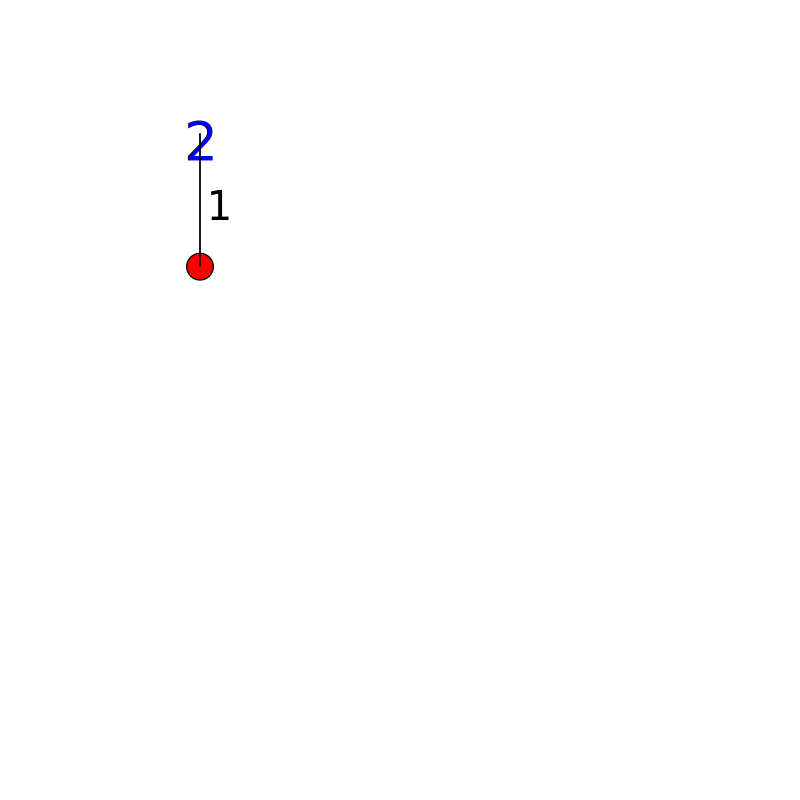
\includegraphics[width=6cm]{../sendmore/FULL/tree_expanded_2}
\end{frame}

\begin{figure}[ht]
\caption{\label{sendmore:Step 1}Search Tree Step 1}
\begin{center}
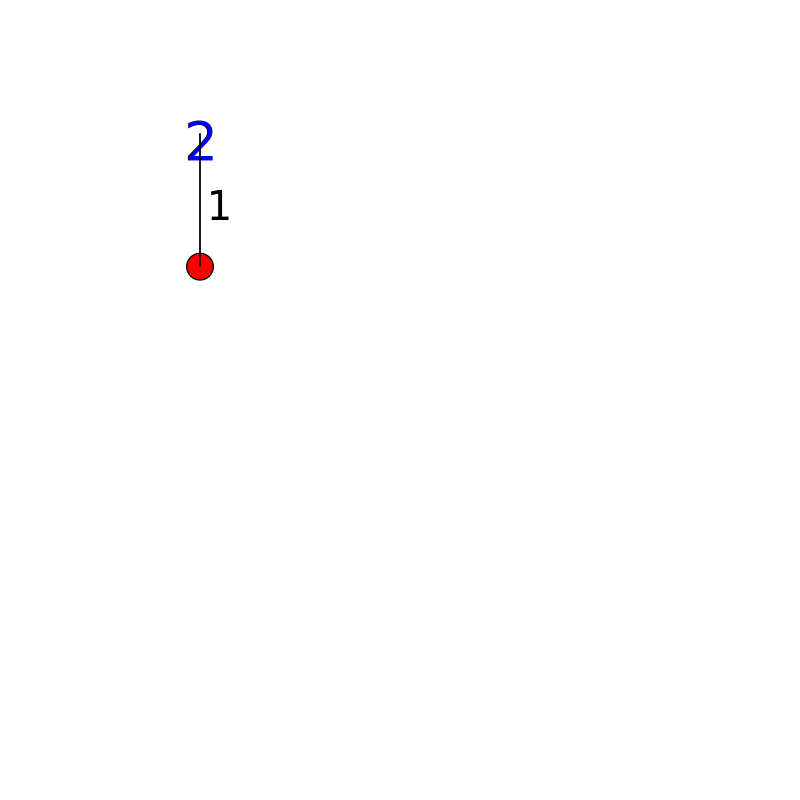
\includegraphics[width=6cm]{../sendmore/FULL/tree_expanded_2}
\end{center}
\end{figure}

Figure~\ref{sendmore:Step 1} shows the search tree at this point. The top node shows the variable being assigned (here $S$), the label on the edge shows the value that is taken (here 9). The link is dotted, as the variable is already assigned, and no new choice is required.

\subsection{Step 2}

\begin{frame}<presentation>
\frametitle{Step 2, Alternative $E=4$}
Variable $E\in \{4..7\}$, first value tested is 4
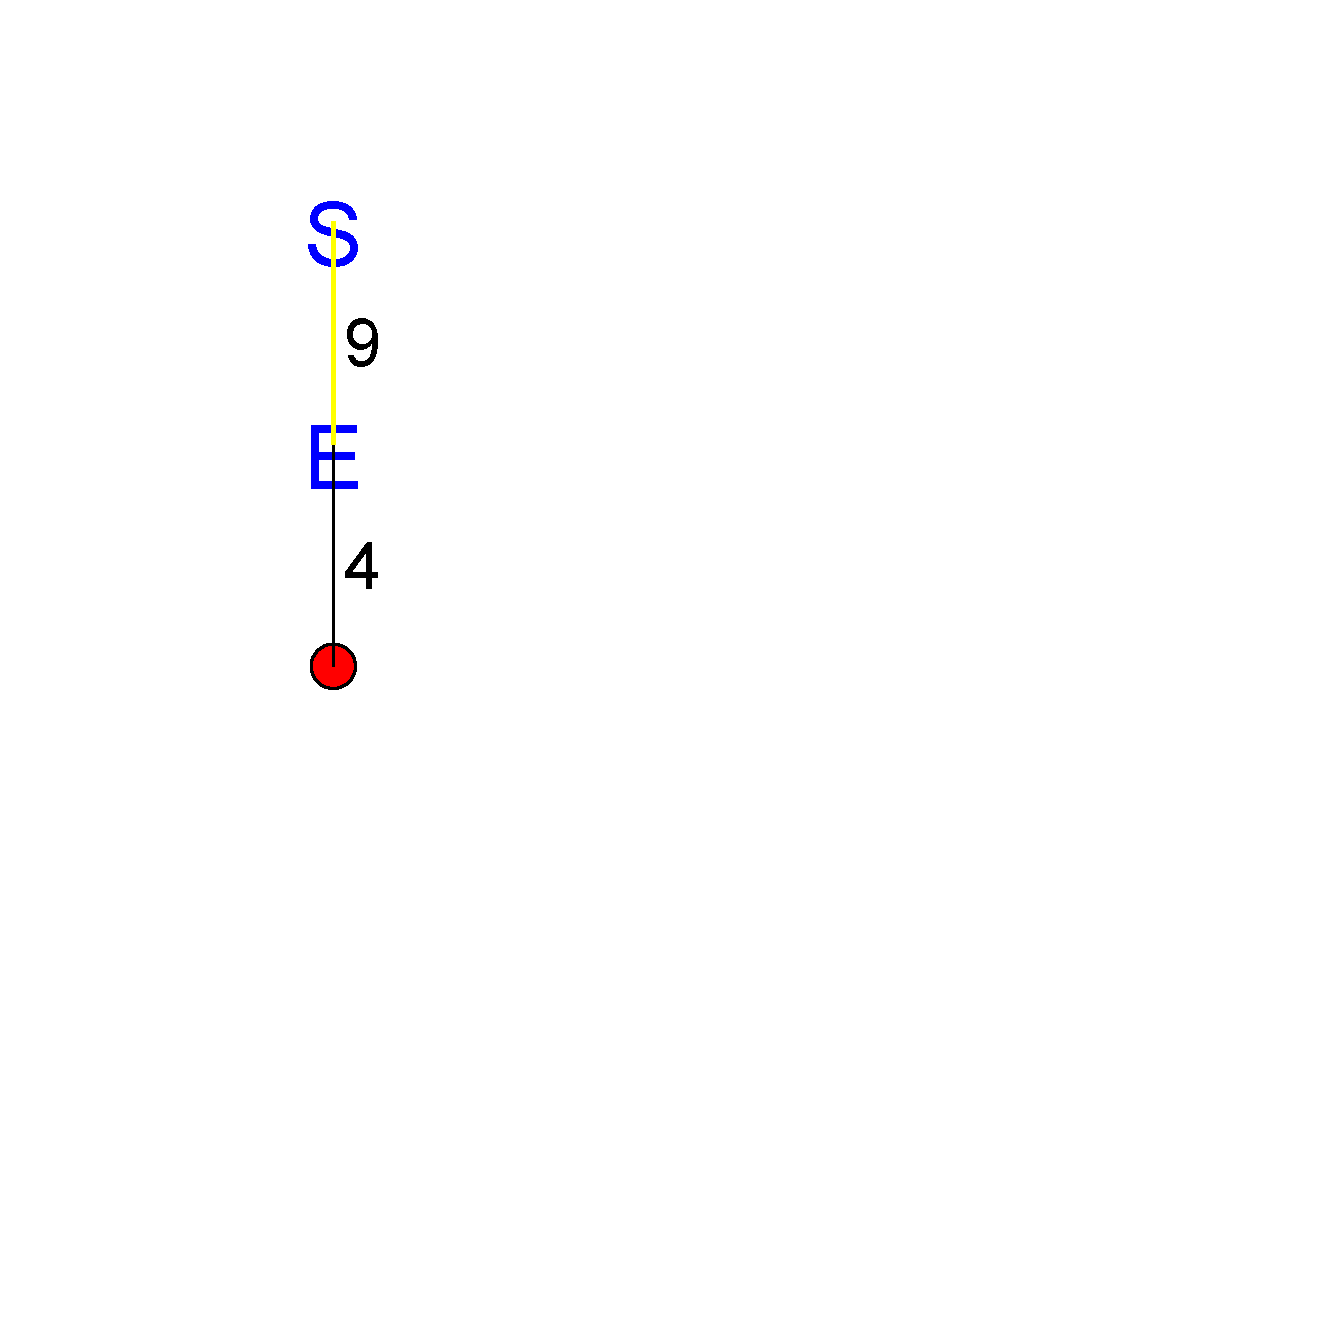
\includegraphics[width=6cm]{../sendmore/FULL/tree_expanded_3}
\end{frame}

\begin{figure}[ht]
\caption{\label{sendmore:Step 2, Alternative 1}Step 2, Alternative $E=4$}
\begin{center}
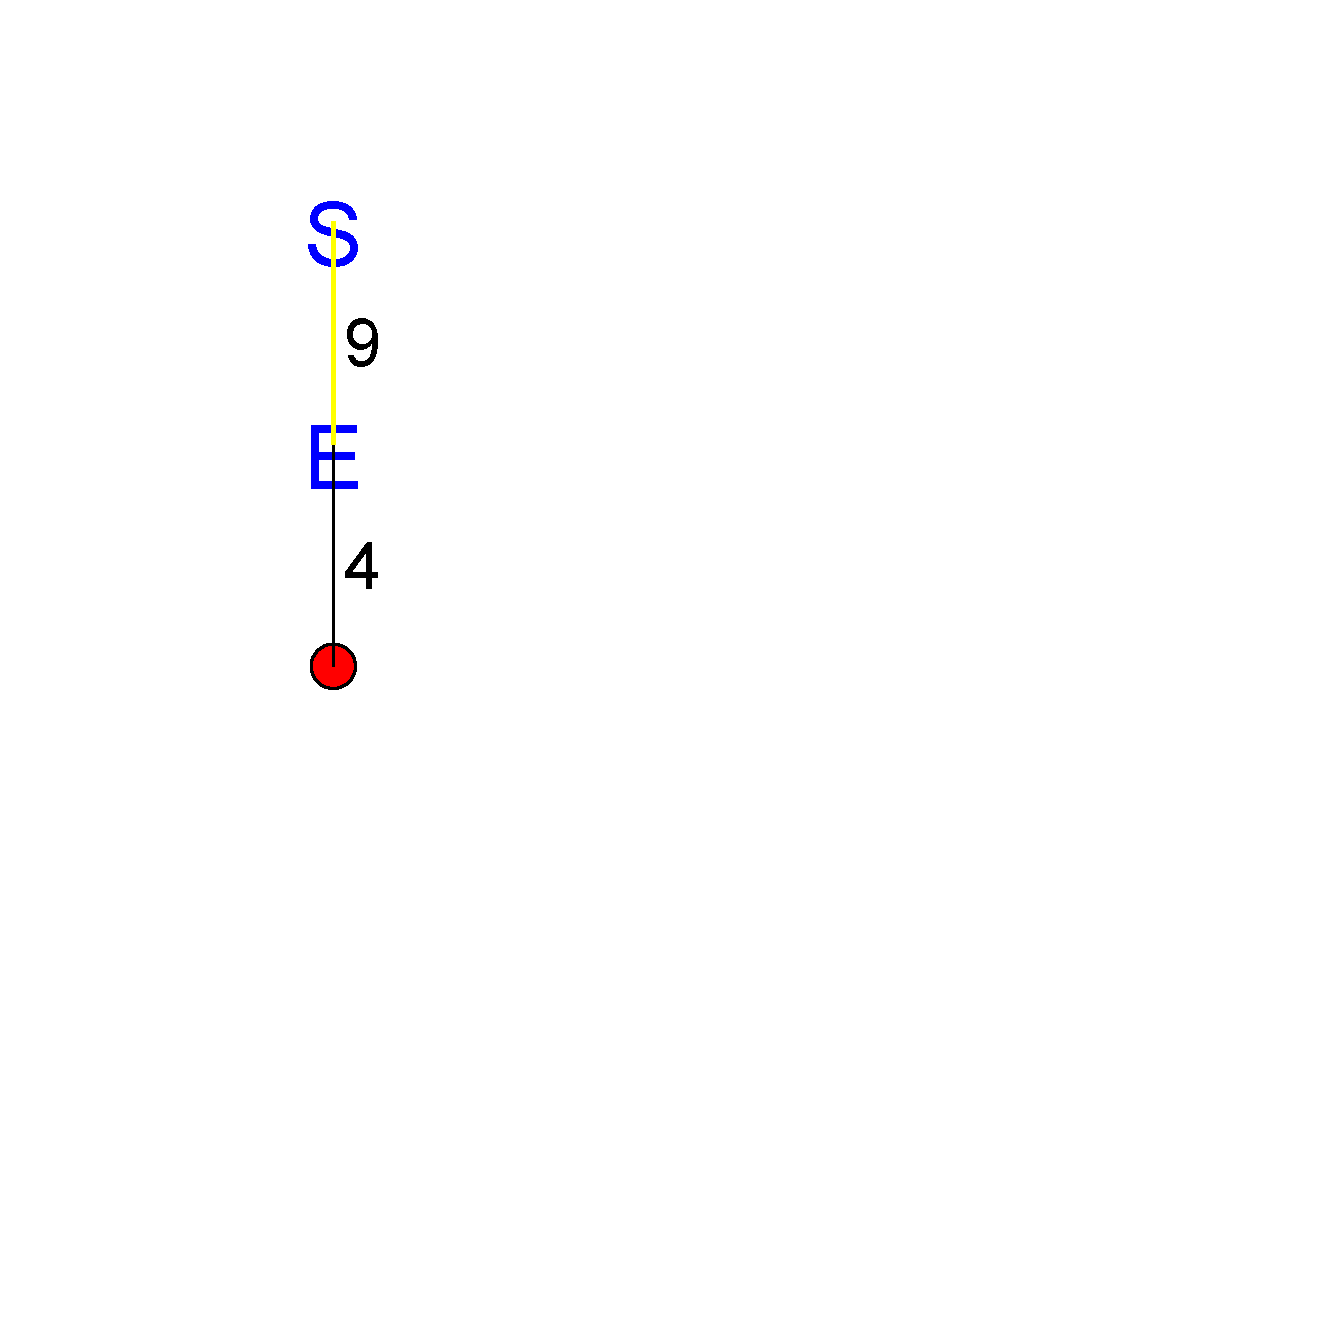
\includegraphics[width=6cm]{../sendmore/FULL/tree_expanded_3}
\end{center}
\end{figure}

Figure~\ref{sendmore:Step 2, Alternative 1} shows the search tree at this point. We are currently assigning variable $E$ to value 4. As this is a proper choice, a solid link is used.

Assigning $E$ to 4 (Figure~\ref{sendmore:assignmente4}) will wake the equality constraint


\begin{frame}<presentation>
\frametitle{Assignment $E=4$}
\begin{center}
\begin{tabular}{|c|c|c|c|c|c|c|c|c|c|c|}\hline
  & 0 & 1 & 2 & 3 & 4 & 5 & 6 & 7 & 8 & 9 \\ \hline
S &\G &\G &\G &\G &\G &\G &\G &\G &\G &\A \\ \hline
E &\G &\G &\G &\G &\F &\X &\X &\X &\G &\G \\ \hline
N &\G &\G &\G &\G &\G &   &   &   &   &\G \\ \hline
D &\G &\G &   &   &   &   &   &   &   &\G \\ \hline
M &\G &\A &\G &\G &\G &\G &\G &\G &\G &\G \\ \hline
O &\A &\G &\G &\G &\G &\G &\G &\G &\G &\G \\ \hline
R &\G &\G &   &   &   &   &   &   &   &\G \\ \hline
Y & \G&\G &   &   &   &   &   &   &   &\G \\ \hline
\end{tabular}

\end{center}
\end{frame}

\begin{figure}[ht]
\caption{\label{sendmore:assignmente4}Assignment $E=4$}
\begin{center}
\begin{tabular}{|c|c|c|c|c|c|c|c|c|c|c|}\hline
  & 0 & 1 & 2 & 3 & 4 & 5 & 6 & 7 & 8 & 9 \\ \hline
S &\G &\G &\G &\G &\G &\G &\G &\G &\G &\A \\ \hline
E &\G &\G &\G &\G &\F &\X &\X &\X &\G &\G \\ \hline
N &\G &\G &\G &\G &\G &   &   &   &   &\G \\ \hline
D &\G &\G &   &   &   &   &   &   &   &\G \\ \hline
M &\G &\A &\G &\G &\G &\G &\G &\G &\G &\G \\ \hline
O &\A &\G &\G &\G &\G &\G &\G &\G &\G &\G \\ \hline
R &\G &\G &   &   &   &   &   &   &   &\G \\ \hline
Y & \G&\G &   &   &   &   &   &   &   &\G \\ \hline
\end{tabular}

\end{center}
\end{figure}


\begin{frame}
\frametitle{Propagation of $E=4$, equality constraint}
\only<1>{
\[
91*4+10*R^{2..8}+D^{2..8} = 90*N^{5..8}+Y^{2..8}
\]
}
\only<2>{
\[
\underbrace{91*4+10*R^{2..8}+D^{2..8}}_{386..452} = \underbrace{90*N^{5..8}+Y^{2..8}}_{452..728}
\]
}
\only<3->{
\[
\underbrace{91*4+10*R^{2..8}+D^{2..8} = 90*N^{5..8}+Y^{2..8}}_{452}
\]
}
\only<4->{
\[
N = 5, Y = 2, R = 8, D = 8
\]
}
\end{frame}

\begin{frame}<presentation>
\frametitle{Result of equality propagation}
\begin{center}
\begin{tabular}{|c|c|c|c|c|c|c|c|c|c|c|}\hline
  & 0 & 1 & 2 & 3 & 4 & 5 & 6 & 7 & 8 & 9 \\ \hline
S &\G &\G &\G &\G &\G &\G &\G &\G &\G &\A \\ \hline
E &\G &\G &\G &\G &\A &\G &\G &\G &\G &\G \\ \hline
N &\G &\G &\G &\G &\G &\F &\X &\X &\X &\G \\ \hline
D &\G &\G &\X &\X &\X &\X &\X &\X &\F &\G \\ \hline
M &\G &\A &\G &\G &\G &\G &\G &\G &\G &\G \\ \hline
O &\A &\G &\G &\G &\G &\G &\G &\G &\G &\G \\ \hline
R &\G &\G &\X &\X &\X &\X &\X &\X &\F &\G \\ \hline
Y & \G&\G &\F &\X &\X &\X &\X &\X &\X &\G \\ \hline
\end{tabular}

\end{center}
\end{frame}

\begin{figure}[ht]
\caption{\label{sendmore:equality1}Result of equality propagation}
\begin{center}
\begin{tabular}{|c|c|c|c|c|c|c|c|c|c|c|}\hline
  & 0 & 1 & 2 & 3 & 4 & 5 & 6 & 7 & 8 & 9 \\ \hline
S &\G &\G &\G &\G &\G &\G &\G &\G &\G &\A \\ \hline
E &\G &\G &\G &\G &\A &\G &\G &\G &\G &\G \\ \hline
N &\G &\G &\G &\G &\G &\F &\X &\X &\X &\G \\ \hline
D &\G &\G &\X &\X &\X &\X &\X &\X &\F &\G \\ \hline
M &\G &\A &\G &\G &\G &\G &\G &\G &\G &\G \\ \hline
O &\A &\G &\G &\G &\G &\G &\G &\G &\G &\G \\ \hline
R &\G &\G &\X &\X &\X &\X &\X &\X &\F &\G \\ \hline
Y & \G&\G &\F &\X &\X &\X &\X &\X &\X &\G \\ \hline
\end{tabular}

\end{center}
\end{figure}

The state after propagation the equality constraint is shown in Figure~\ref{sendmore:equality1}.

\begin{frame}<presentation>
\frametitle{Propagation of alldifferent}
\begin{center}
\only<beamer>{
\only<1>{
\begin{tabular}{|c|c|c|c|c|c|c|c|c|c|c|}\hline
  & 0 & 1 & 2 & 3 & 4 & 5 & 6 & 7 & 8 & 9 \\ \hline
S &\G &\G &\G &\G &\G &\G &\G &\G &\G &\A \\ \hline
E &\G &\G &\G &\G &\A &\G &\G &\G &\G &\G \\ \hline
N &\G &\G &\G &\G &\G &\F &\X &\X &\X &\G \\ \hline
D &\G &\G &\X &\X &\X &\X &\X &\X &\F &\G \\ \hline
M &\G &\A &\G &\G &\G &\G &\G &\G &\G &\G \\ \hline
O &\A &\G &\G &\G &\G &\G &\G &\G &\G &\G \\ \hline
R &\G &\G &\X &\X &\X &\X &\X &\X &\F &\G \\ \hline
Y & \G&\G &\F &\X &\X &\X &\X &\X &\X &\G \\ \hline
\end{tabular}
}
}
\only<2>{
\begin{tabular}{|c|c|c|c|c|c|c|c|c|c|c|}\hline
  & 0 & 1 & 2 & 3 & 4 & 5 & 6 & 7 & 8 & 9 \\ \hline
S &\G &\G &\G &\G &\G &\G &\G &\G &\Y &\A \\ \hline
E &\G &\G &\G &\G &\A &\G &\G &\G &\Y &\G \\ \hline
N &\G &\G &\G &\G &\G &\F &\X &\X &\Y &\G \\ \hline
D &\G &\G &\X &\X &\X &\X &\X &\X &\F &\G \\ \hline
M &\G &\A &\G &\G &\G &\G &\G &\G &\Y &\G \\ \hline
O &\A &\G &\G &\G &\G &\G &\G &\G &\Y &\G \\ \hline
R &\G &\G &\X &\X &\X &\X &\X &\X &\F &\G \\ \hline
Y & \G&\G &\F &\X &\X &\X &\X &\X &\Y &\G \\ \hline
\end{tabular}
}
\end{center}
\only<2>{\alert<2>{Alldifferent fails!}}
\end{frame}

\begin{figure}[ht]
\caption{\label{sendmore:alldifferentprop2}Propagation of \texttt{alldifferent} fails!}
\begin{center}
\begin{tabular}{|c|c|c|c|c|c|c|c|c|c|c|}\hline
  & 0 & 1 & 2 & 3 & 4 & 5 & 6 & 7 & 8 & 9 \\ \hline
S &\G &\G &\G &\G &\G &\G &\G &\G &\Y &\A \\ \hline
E &\G &\G &\G &\G &\A &\G &\G &\G &\Y &\G \\ \hline
N &\G &\G &\G &\G &\G &\F &\X &\X &\Y &\G \\ \hline
D &\G &\G &\X &\X &\X &\X &\X &\X &\F &\G \\ \hline
M &\G &\A &\G &\G &\G &\G &\G &\G &\Y &\G \\ \hline
O &\A &\G &\G &\G &\G &\G &\G &\G &\Y &\G \\ \hline
R &\G &\G &\X &\X &\X &\X &\X &\X &\F &\G \\ \hline
Y & \G&\G &\F &\X &\X &\X &\X &\X &\Y &\G \\ \hline
\end{tabular}

\end{center}
\end{figure}


The assignments will trigger the \texttt{alldifferent} constraint, but the constraint detects that two variables ($D$ and $R$) have the same value 8. This is not allowed and the \texttt{alldifferent} constraint fails (Figure~\ref{sendmore:alldifferentprop2}).

\begin{frame}<presentation>
\frametitle{Step 2, Alternative $E = 5$}
Return to last open choice, $E$, and test next value
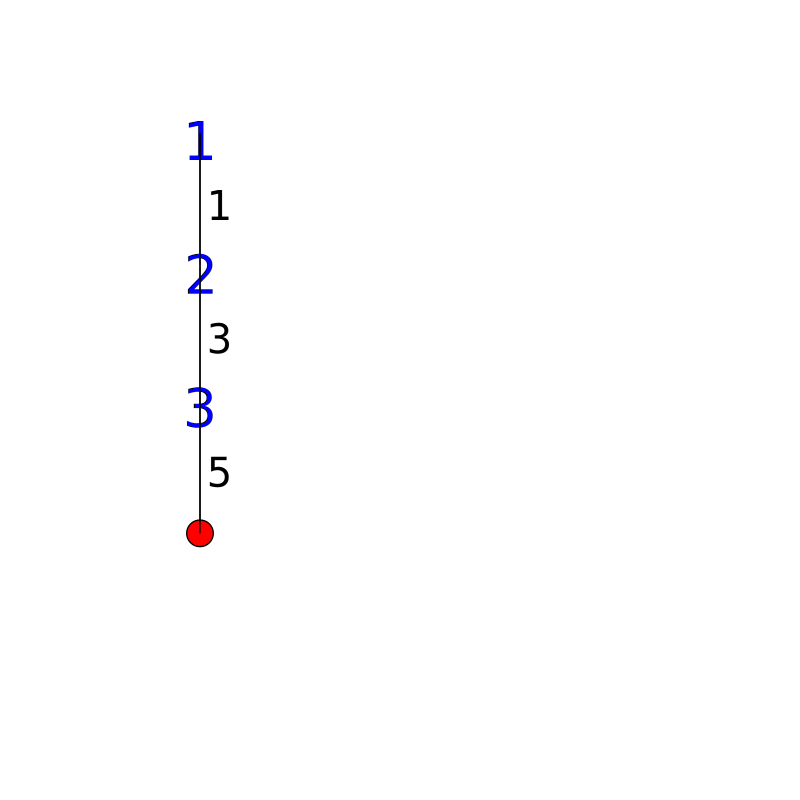
\includegraphics[width=6cm]{../sendmore/FULL/tree_expanded_4}
\end{frame}

\begin{figure}[ht]
\caption{\label{sendmore:Step 2, Alternative 2}Step 2, Alternative $E = 5$}
\begin{center}
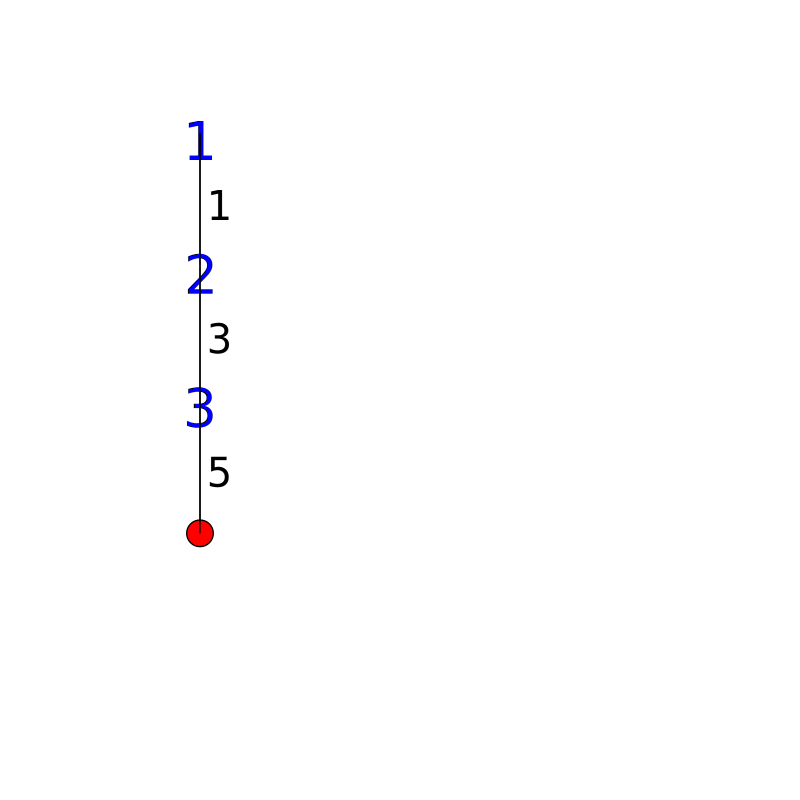
\includegraphics[width=6cm]{../sendmore/FULL/tree_expanded_4}
\end{center}
\end{figure}

We backtrack\index{backtrack} to the last choice ($E$), and then try the next value ($E = 5$). This situation is depicted in figure~\ref{sendmore:Step 2, Alternative 2}. The left child of node $E$ is marked as a failure, we are currently testing value 5, the second alternative.
The assignment of value ($E=5$) will trigger both the \texttt{alldifferent} and the equality constraint. Assume that the \texttt{alldifferent} is woken first\footnote{Which of the constraints is woken up first can be difficult to predict without understanding the details of the implementation of the solver}.

\begin{frame}<presentation>
\frametitle{Assignment $E=5$}
\begin{center}
\begin{tabular}{|c|c|c|c|c|c|c|c|c|c|c|}\hline
  & 0 & 1 & 2 & 3 & 4 & 5 & 6 & 7 & 8 & 9 \\ \hline
S &\G &\G &\G &\G &\G &\G &\G &\G &\G &\A \\ \hline
E &\G &\G &\G &\G &\X &\F &\X &\X &\G &\G \\ \hline
N &\G &\G &\G &\G &\G &   &   &   &   &\G \\ \hline
D &\G &\G &   &   &   &   &   &   &   &\G \\ \hline
M &\G &\A &\G &\G &\G &\G &\G &\G &\G &\G \\ \hline
O &\A &\G &\G &\G &\G &\G &\G &\G &\G &\G \\ \hline
R &\G &\G &   &   &   &   &   &   &   &\G \\ \hline
Y & \G&\G &   &   &   &   &   &   &   &\G \\ \hline
\end{tabular}

\end{center}
\end{frame}

\begin{figure}[ht]
\caption{\label{sendmore:assignmente5}Assignment $E=5$}
\begin{center}
\begin{tabular}{|c|c|c|c|c|c|c|c|c|c|c|}\hline
  & 0 & 1 & 2 & 3 & 4 & 5 & 6 & 7 & 8 & 9 \\ \hline
S &\G &\G &\G &\G &\G &\G &\G &\G &\G &\A \\ \hline
E &\G &\G &\G &\G &\X &\F &\X &\X &\G &\G \\ \hline
N &\G &\G &\G &\G &\G &   &   &   &   &\G \\ \hline
D &\G &\G &   &   &   &   &   &   &   &\G \\ \hline
M &\G &\A &\G &\G &\G &\G &\G &\G &\G &\G \\ \hline
O &\A &\G &\G &\G &\G &\G &\G &\G &\G &\G \\ \hline
R &\G &\G &   &   &   &   &   &   &   &\G \\ \hline
Y & \G&\G &   &   &   &   &   &   &   &\G \\ \hline
\end{tabular}

\end{center}
\end{figure}



\begin{frame}<presentation>
\frametitle{Propagation of alldifferent}
\begin{center}
\only<beamer>{
\only<1>{
\begin{tabular}{|c|c|c|c|c|c|c|c|c|c|c|}\hline
  & 0 & 1 & 2 & 3 & 4 & 5 & 6 & 7 & 8 & 9 \\ \hline
S &\G &\G &\G &\G &\G &\G &\G &\G &\G &\A \\ \hline
E &\G &\G &\G &\G &\X &\F &\X &\X &\G &\G \\ \hline
N &\G &\G &\G &\G &\G &   &   &   &   &\G \\ \hline
D &\G &\G &   &   &   &   &   &   &   &\G \\ \hline
M &\G &\A &\G &\G &\G &\G &\G &\G &\G &\G \\ \hline
O &\A &\G &\G &\G &\G &\G &\G &\G &\G &\G \\ \hline
R &\G &\G &   &   &   &   &   &   &   &\G \\ \hline
Y & \G&\G &   &   &   &   &   &   &   &\G \\ \hline
\end{tabular}
}
\only<2>{
\begin{tabular}{|c|c|c|c|c|c|c|c|c|c|c|}\hline
  & 0 & 1 & 2 & 3 & 4 & 5 & 6 & 7 & 8 & 9 \\ \hline
S &\G &\G &\G &\G &\G &\G &\G &\G &\G &\A \\ \hline
E &\G &\G &\G &\G &\G &\F &\G &\G &\G &\G \\ \hline
N &\G &\G &\G &\G &\G &\D &   &   &   &\G \\ \hline
D &\G &\G &   &   &   &\D &   &   &   &\G \\ \hline
M &\G &\A &\G &\G &\G &\G &\G &\G &\G &\G \\ \hline
O &\A &\G &\G &\G &\G &\G &\G &\G &\G &\G \\ \hline
R &\G &\G &   &   &   &\D &   &   &   &\G \\ \hline
Y & \G&\G &   &   &   &\D &   &   &   &\G \\ \hline
\end{tabular}
}
}
\only<3>{
\begin{tabular}{|c|c|c|c|c|c|c|c|c|c|c|}\hline
  & 0 & 1 & 2 & 3 & 4 & 5 & 6 & 7 & 8 & 9 \\ \hline
S &\G &\G &\G &\G &\G &\G &\G &\G &\G &\A \\ \hline
E &\G &\G &\G &\G &\G &\A &\G &\G &\G &\G \\ \hline
N &\G &\G &\G &\G &\G &\G &   &   &   &\G \\ \hline
D &\G &\G &   &   &   &\G &   &   &   &\G \\ \hline
M &\G &\A &\G &\G &\G &\G &\G &\G &\G &\G \\ \hline
O &\A &\G &\G &\G &\G &\G &\G &\G &\G &\G \\ \hline
R &\G &\G &   &   &   &\G &   &   &   &\G \\ \hline
Y & \G&\G &   &   &   &\G &   &   &   &\G \\ \hline
\end{tabular}

}
\end{center}
\only<3>{
\[
N \neq 5, N \geq 6
\]
}
\end{frame}

\begin{figure}[ht]
\caption{\label{sendmore:alldifferentprop3}Propagation of \texttt{alldifferent}}
\begin{center}
\begin{tabular}{|c|c|c|c|c|c|c|c|c|c|c|}\hline
  & 0 & 1 & 2 & 3 & 4 & 5 & 6 & 7 & 8 & 9 \\ \hline
S &\G &\G &\G &\G &\G &\G &\G &\G &\G &\A \\ \hline
E &\G &\G &\G &\G &\G &\A &\G &\G &\G &\G \\ \hline
N &\G &\G &\G &\G &\G &\G &   &   &   &\G \\ \hline
D &\G &\G &   &   &   &\G &   &   &   &\G \\ \hline
M &\G &\A &\G &\G &\G &\G &\G &\G &\G &\G \\ \hline
O &\A &\G &\G &\G &\G &\G &\G &\G &\G &\G \\ \hline
R &\G &\G &   &   &   &\G &   &   &   &\G \\ \hline
Y & \G&\G &   &   &   &\G &   &   &   &\G \\ \hline
\end{tabular}

\end{center}
\end{figure}


The propagation of the assignment $E=5$ in the \texttt{alldifferent} constraint will remove value 5 from the variable $N$ (Figure~\ref{sendmore:alldifferentprop3}). At this point, since the lower bound of variable $N$ is updated to 6, the equality constraint is triggered.

\begin{frame}
\frametitle{Propagation of equality}
\only<1>{
\[
91*5+10*R^{2..8}+D^{2..8} = 90*N^{6..8}+Y^{2..8}
\]
}
\only<2>{
\[
\underbrace{91*5+10*R^{2..8}+D^{2..8}}_{477..543} = \underbrace{90*N^{6..8}+Y^{2..8}}_{542..728}
\]
}
\only<3->{
\[
\underbrace{91*5+10*R^{2..8}+D^{2..8} = 90*N^{6..8}+Y^{2..8}}_{542..543}
\]
}
\only<4>{
\[
N = 6, Y \in \{2,3\}, R = 8, D \in \{7..8\}
\]
}
\end{frame}

\begin{frame}<presentation>
\frametitle{Result of equality propagation}
\begin{center}
\begin{tabular}{|c|c|c|c|c|c|c|c|c|c|c|}\hline
  & 0 & 1 & 2 & 3 & 4 & 5 & 6 & 7 & 8 & 9 \\ \hline
S &\G &\G &\G &\G &\G &\G &\G &\G &\G &\A \\ \hline
E &\G &\G &\G &\G &\G &\A &\G &\G &\G &\G \\ \hline
N &\G &\G &\G &\G &\G &\G &\F &\X &\X &\G \\ \hline
D &\G &\G &\R &\R &\R &\G &\R &   &   &\G \\ \hline
M &\G &\A &\G &\G &\G &\G &\G &\G &\G &\G \\ \hline
O &\A &\G &\G &\G &\G &\G &\G &\G &\G &\G \\ \hline
R &\G &\G &\X &\X &\X &\G &\X &\X &\F &\G \\ \hline
Y & \G&\G &   &   &\R &\G &\R &\R &\R &\G \\ \hline
\end{tabular}

\end{center}
\end{frame}

\begin{figure}[ht]
\caption{\label{sendmore:equality2}Result of equality propagation}
\begin{center}
\begin{tabular}{|c|c|c|c|c|c|c|c|c|c|c|}\hline
  & 0 & 1 & 2 & 3 & 4 & 5 & 6 & 7 & 8 & 9 \\ \hline
S &\G &\G &\G &\G &\G &\G &\G &\G &\G &\A \\ \hline
E &\G &\G &\G &\G &\G &\A &\G &\G &\G &\G \\ \hline
N &\G &\G &\G &\G &\G &\G &\F &\X &\X &\G \\ \hline
D &\G &\G &\R &\R &\R &\G &\R &   &   &\G \\ \hline
M &\G &\A &\G &\G &\G &\G &\G &\G &\G &\G \\ \hline
O &\A &\G &\G &\G &\G &\G &\G &\G &\G &\G \\ \hline
R &\G &\G &\X &\X &\X &\G &\X &\X &\F &\G \\ \hline
Y & \G&\G &   &   &\R &\G &\R &\R &\R &\G \\ \hline
\end{tabular}

\end{center}
\end{figure}


\begin{frame}<presentation>
\frametitle{Propagation of \texttt{alldifferent}}
\begin{center}
\only<beamer>{
\only<1>{
\begin{tabular}{|c|c|c|c|c|c|c|c|c|c|c|}\hline
  & 0 & 1 & 2 & 3 & 4 & 5 & 6 & 7 & 8 & 9 \\ \hline
S &\G &\G &\G &\G &\G &\G &\G &\G &\G &\A \\ \hline
E &\G &\G &\G &\G &\G &\A &\G &\G &\G &\G \\ \hline
N &\G &\G &\G &\G &\G &\G &\F &\X &\X &\G \\ \hline
D &\G &\G &\R &\R &\R &\G &\R &   &   &\G \\ \hline
M &\G &\A &\G &\G &\G &\G &\G &\G &\G &\G \\ \hline
O &\A &\G &\G &\G &\G &\G &\G &\G &\G &\G \\ \hline
R &\G &\G &\X &\X &\X &\G &\X &\X &\F &\G \\ \hline
Y & \G&\G &   &   &\R &\G &\R &\R &\R &\G \\ \hline
\end{tabular}
}
\only<2>{
\begin{tabular}{|c|c|c|c|c|c|c|c|c|c|c|}\hline
  & 0 & 1 & 2 & 3 & 4 & 5 & 6 & 7 & 8 & 9 \\ \hline
S &\G &\G &\G &\G &\G &\G &\G &\G &\G &\A \\ \hline
E &\G &\G &\G &\G &\G &\A &\G &\G &\G &\G \\ \hline
N &\G &\G &\G &\G &\G &\G &\A &\G &\G &\G \\ \hline
D &\G &\G &\G &\G &\G &\G &\G &   &\D &\G \\ \hline
M &\G &\A &\G &\G &\G &\G &\G &\G &\G &\G \\ \hline
O &\A &\G &\G &\G &\G &\G &\G &\G &\G &\G \\ \hline
R &\G &\G &\G &\G &\G &\G &\G &\G &\F &\G \\ \hline
Y & \G&\G &   &   &\G &\G &\G &\G &\G &\G \\ \hline
\end{tabular}
}
\only<3>{
\begin{tabular}{|c|c|c|c|c|c|c|c|c|c|c|}\hline
  & 0 & 1 & 2 & 3 & 4 & 5 & 6 & 7 & 8 & 9 \\ \hline
S &\G &\G &\G &\G &\G &\G &\G &\G &\G &\A \\ \hline
E &\G &\G &\G &\G &\G &\A &\G &\G &\G &\G \\ \hline
N &\G &\G &\G &\G &\G &\G &\A &\G &\G &\G \\ \hline
D &\G &\G &\G &\G &\G &\G &\G &\F &\G &\G \\ \hline
M &\G &\A &\G &\G &\G &\G &\G &\G &\G &\G \\ \hline
O &\A &\G &\G &\G &\G &\G &\G &\G &\G &\G \\ \hline
R &\G &\G &\G &\G &\G &\G &\G &\G &\A &\G \\ \hline
Y & \G&\G &   &   &\G &\G &\G &\G &\G &\G \\ \hline
\end{tabular}
}
}
\only<4>{
\begin{tabular}{|c|c|c|c|c|c|c|c|c|c|c|}\hline
  & 0 & 1 & 2 & 3 & 4 & 5 & 6 & 7 & 8 & 9 \\ \hline
S &\G &\G &\G &\G &\G &\G &\G &\G &\G &\A \\ \hline
E &\G &\G &\G &\G &\G &\A &\G &\G &\G &\G \\ \hline
N &\G &\G &\G &\G &\G &\G &\A &\G &\G &\G \\ \hline
D &\G &\G &\G &\G &\G &\G &\G &\A &\G &\G \\ \hline
M &\G &\A &\G &\G &\G &\G &\G &\G &\G &\G \\ \hline
O &\A &\G &\G &\G &\G &\G &\G &\G &\G &\G \\ \hline
R &\G &\G &\G &\G &\G &\G &\G &\G &\A &\G \\ \hline
Y & \G&\G &   &   &\G &\G &\G &\G &\G &\G \\ \hline
\end{tabular}

}
\end{center}
\only<4>{
\[
D = 7
\]
}
\end{frame}

\begin{figure}[ht]
\caption{\label{sendmore:alldifferentprop4}Propagation of \texttt{alldifferent}}
\begin{center}
\begin{tabular}{|c|c|c|c|c|c|c|c|c|c|c|}\hline
  & 0 & 1 & 2 & 3 & 4 & 5 & 6 & 7 & 8 & 9 \\ \hline
S &\G &\G &\G &\G &\G &\G &\G &\G &\G &\A \\ \hline
E &\G &\G &\G &\G &\G &\A &\G &\G &\G &\G \\ \hline
N &\G &\G &\G &\G &\G &\G &\A &\G &\G &\G \\ \hline
D &\G &\G &\G &\G &\G &\G &\G &\A &\G &\G \\ \hline
M &\G &\A &\G &\G &\G &\G &\G &\G &\G &\G \\ \hline
O &\A &\G &\G &\G &\G &\G &\G &\G &\G &\G \\ \hline
R &\G &\G &\G &\G &\G &\G &\G &\G &\A &\G \\ \hline
Y & \G&\G &   &   &\G &\G &\G &\G &\G &\G \\ \hline
\end{tabular}

\end{center}
\end{figure}


The \texttt{alldifferent} constraint (figure~\ref{sendmore:alldifferentprop4}) has fixed variable $D$ to 7. We again wake the equality constraint.

\begin{frame}
\frametitle{Propagation of equality}
\only<1>{
\[
91*5+10*8+7 = 90*6+Y^{2..3}
\]
}
\only<2>{
\[
\underbrace{91*5+10*8+7}_{542} = \underbrace{90*6+Y^{2..3}}_{542..543}
\]
}
\only<3->{
\[
\underbrace{91*5+10*8+7 = 90*6+Y^{2..3}}_{542}
\]
}
\only<4>{
\[
Y = 2
\]
}
\end{frame}

This finally assigns the last variable $Y$ to 2 (Figure~\ref{sendmore:lastprop}).

\begin{frame}<presentation>
\frametitle{Last propagation step}
\begin{center}
\begin{tabular}{|c|c|c|c|c|c|c|c|c|c|c|}\hline
  & 0 & 1 & 2 & 3 & 4 & 5 & 6 & 7 & 8 & 9 \\ \hline
S &\G &\G &\G &\G &\G &\G &\G &\G &\G &\A \\ \hline
E &\G &\G &\G &\G &\G &\A &\G &\G &\G &\G \\ \hline
N &\G &\G &\G &\G &\G &\G &\A &\G &\G &\G \\ \hline
D &\G &\G &\G &\G &\G &\G &\G &\A &\G &\G \\ \hline
M &\G &\A &\G &\G &\G &\G &\G &\G &\G &\G \\ \hline
O &\A &\G &\G &\G &\G &\G &\G &\G &\G &\G \\ \hline
R &\G &\G &\G &\G &\G &\G &\G &\G &\A &\G \\ \hline
Y & \G&\G &\F &\X &\G &\G &\G &\G &\G &\G \\ \hline
\end{tabular}

\end{center}
\end{frame}

\begin{figure}[ht]
\caption{\label{sendmore:lastprop}Last propagation step}
\begin{center}
\begin{tabular}{|c|c|c|c|c|c|c|c|c|c|c|}\hline
  & 0 & 1 & 2 & 3 & 4 & 5 & 6 & 7 & 8 & 9 \\ \hline
S &\G &\G &\G &\G &\G &\G &\G &\G &\G &\A \\ \hline
E &\G &\G &\G &\G &\G &\A &\G &\G &\G &\G \\ \hline
N &\G &\G &\G &\G &\G &\G &\A &\G &\G &\G \\ \hline
D &\G &\G &\G &\G &\G &\G &\G &\A &\G &\G \\ \hline
M &\G &\A &\G &\G &\G &\G &\G &\G &\G &\G \\ \hline
O &\A &\G &\G &\G &\G &\G &\G &\G &\G &\G \\ \hline
R &\G &\G &\G &\G &\G &\G &\G &\G &\A &\G \\ \hline
Y & \G&\G &\F &\X &\G &\G &\G &\G &\G &\G \\ \hline
\end{tabular}

\end{center}
\end{figure}


\subsection{Further Steps}

\begin{frame}<beamer>
\frametitle{Further Steps: Nothing more to do}
\only<1>{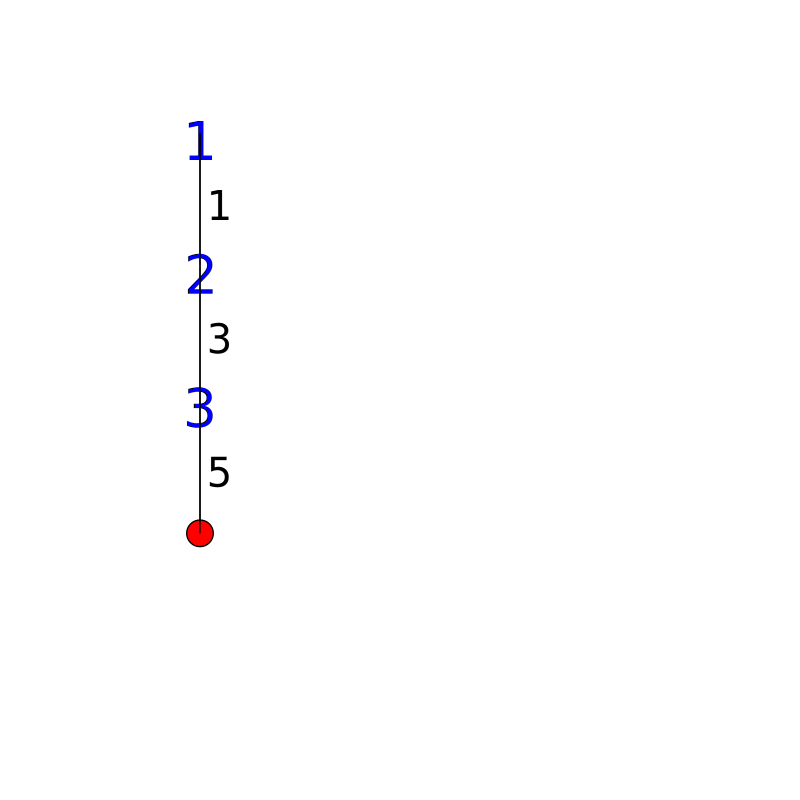
\includegraphics[width=6cm]{../sendmore/FULL/tree_expanded_4}}
\only<2>{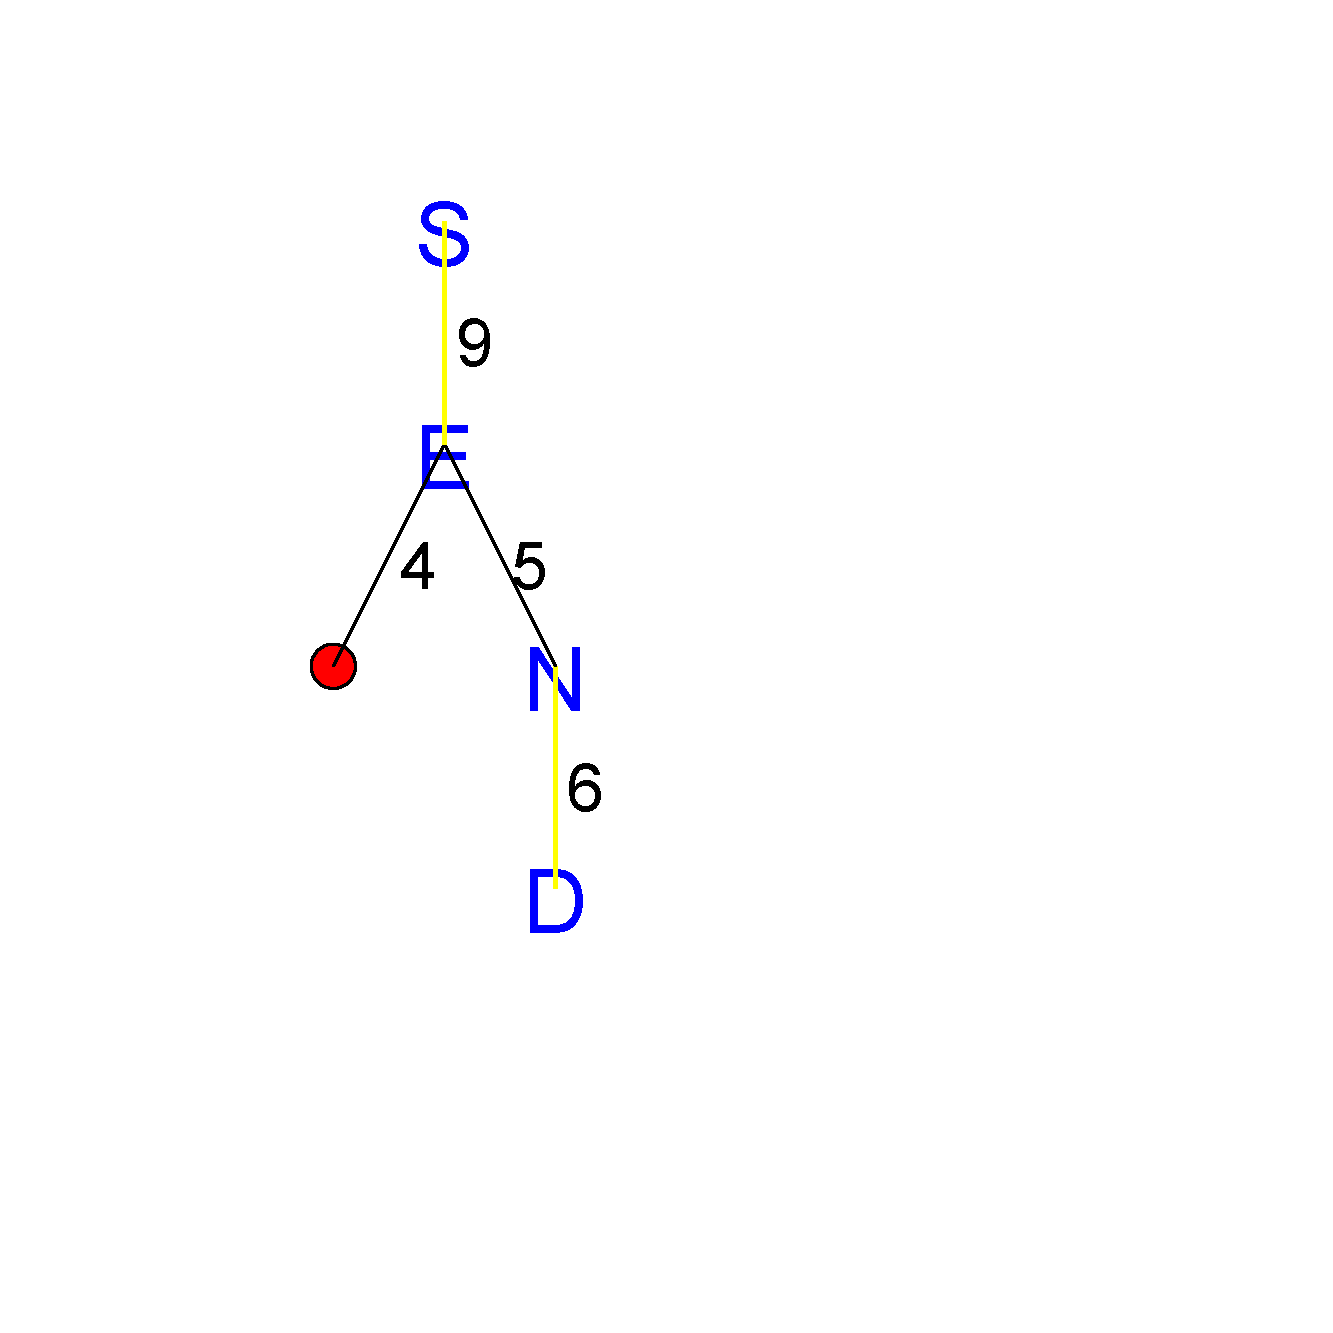
\includegraphics[width=6cm]{../sendmore/FULL/tree_expanded_5}}
\only<3>{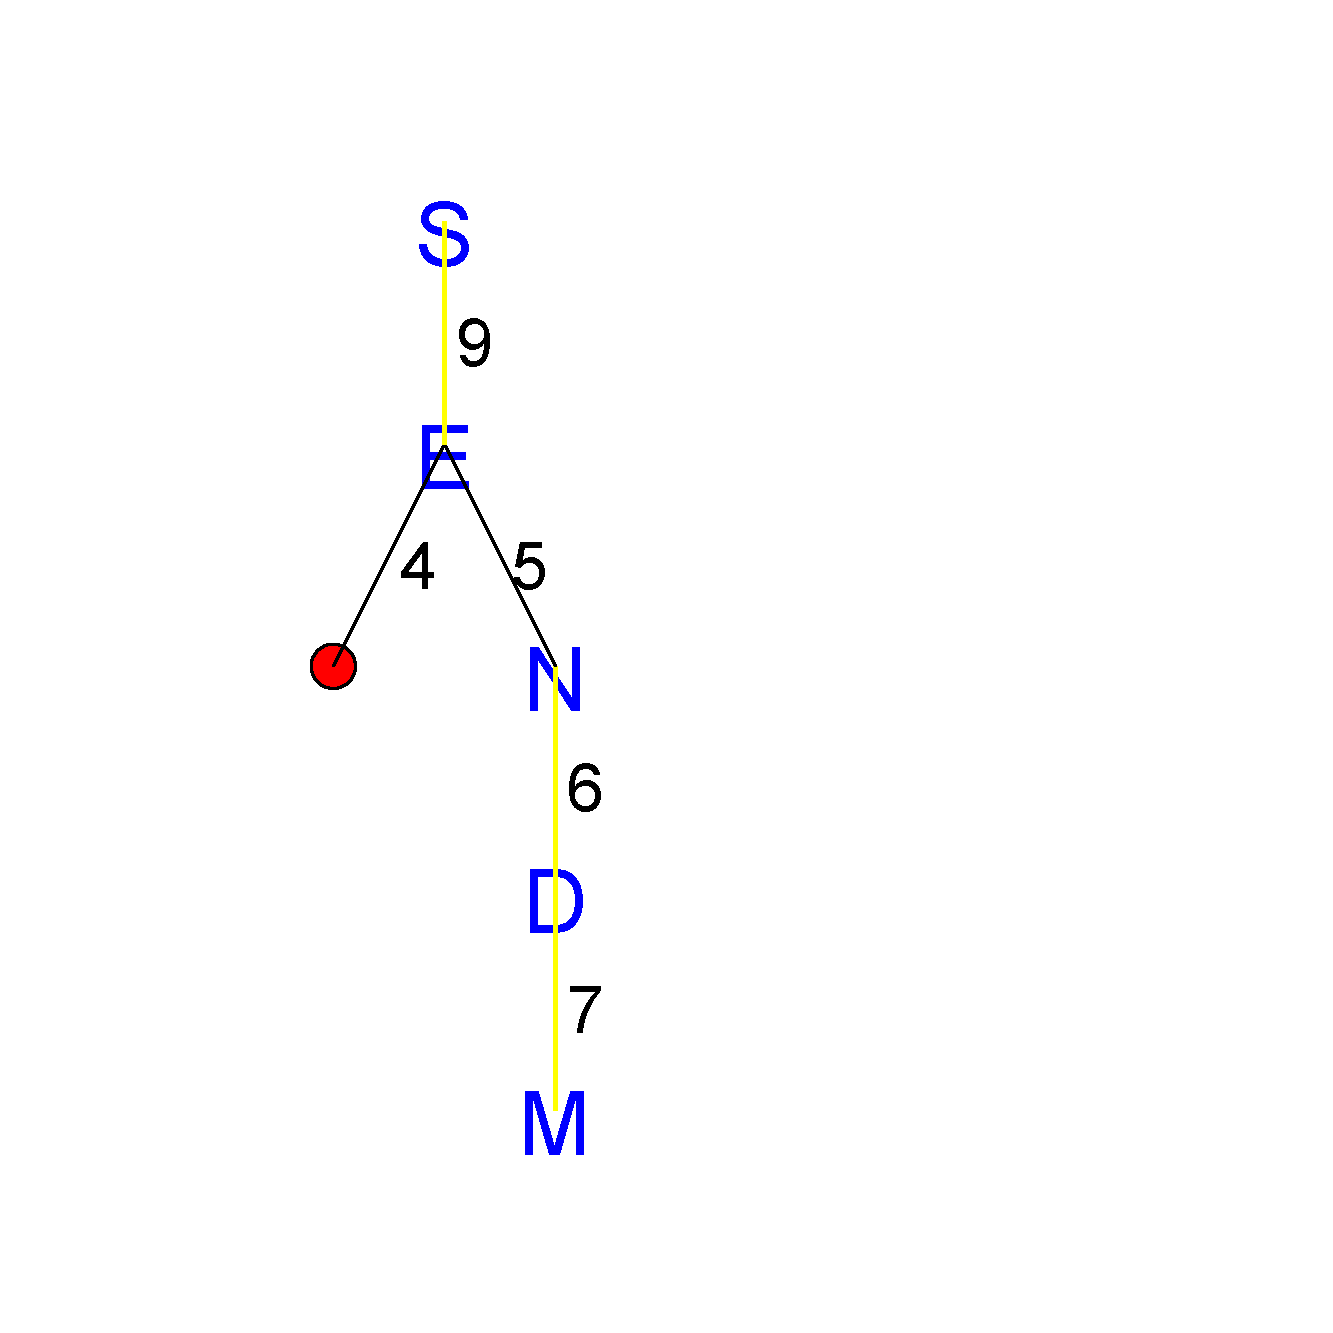
\includegraphics[width=6cm]{../sendmore/FULL/tree_expanded_6}}
\only<4>{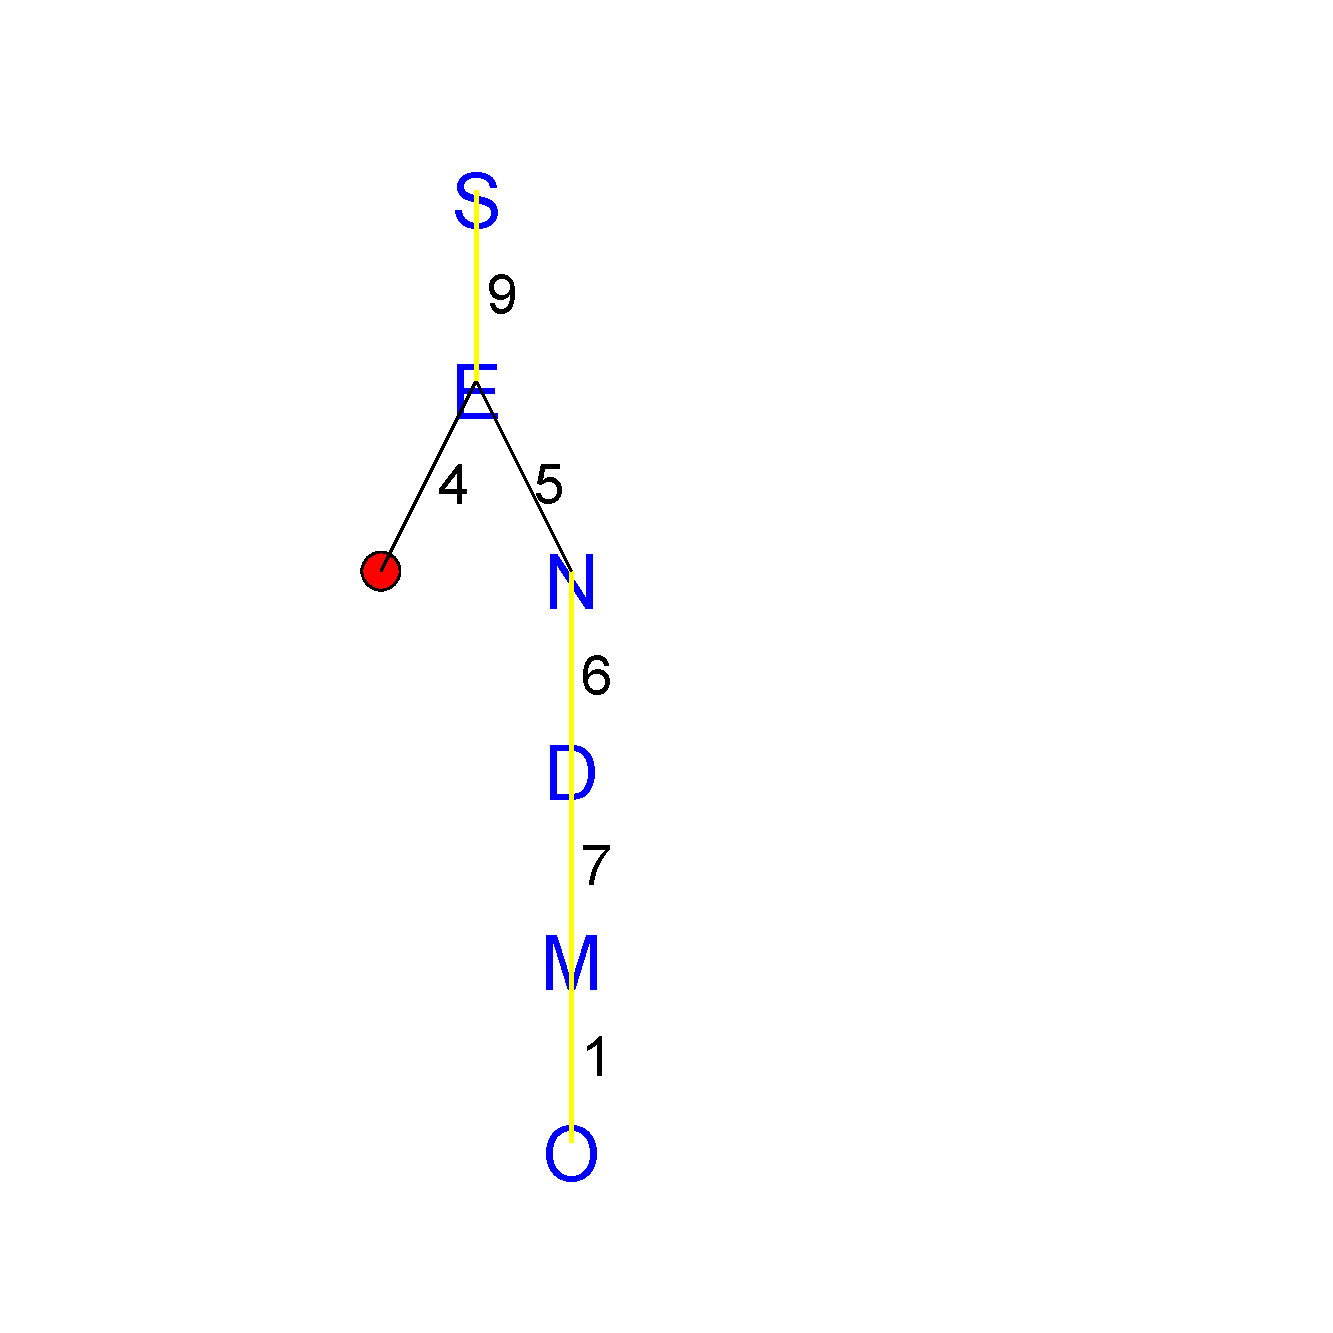
\includegraphics[width=6cm]{../sendmore/FULL/tree_expanded_7}}
\only<5>{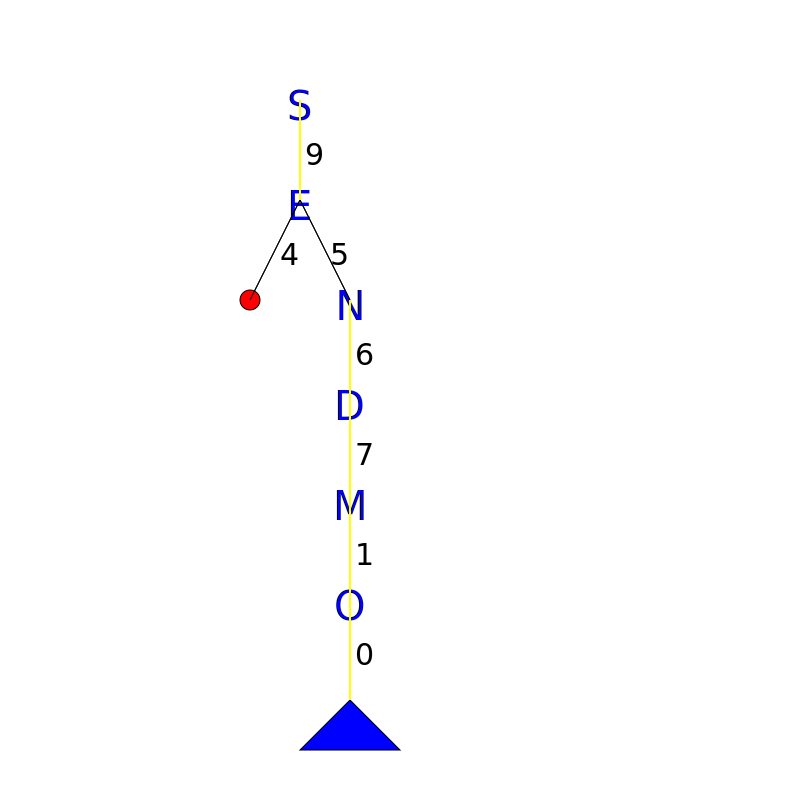
\includegraphics[width=6cm]{../sendmore/FULL/tree_expanded_8}}
\only<6>{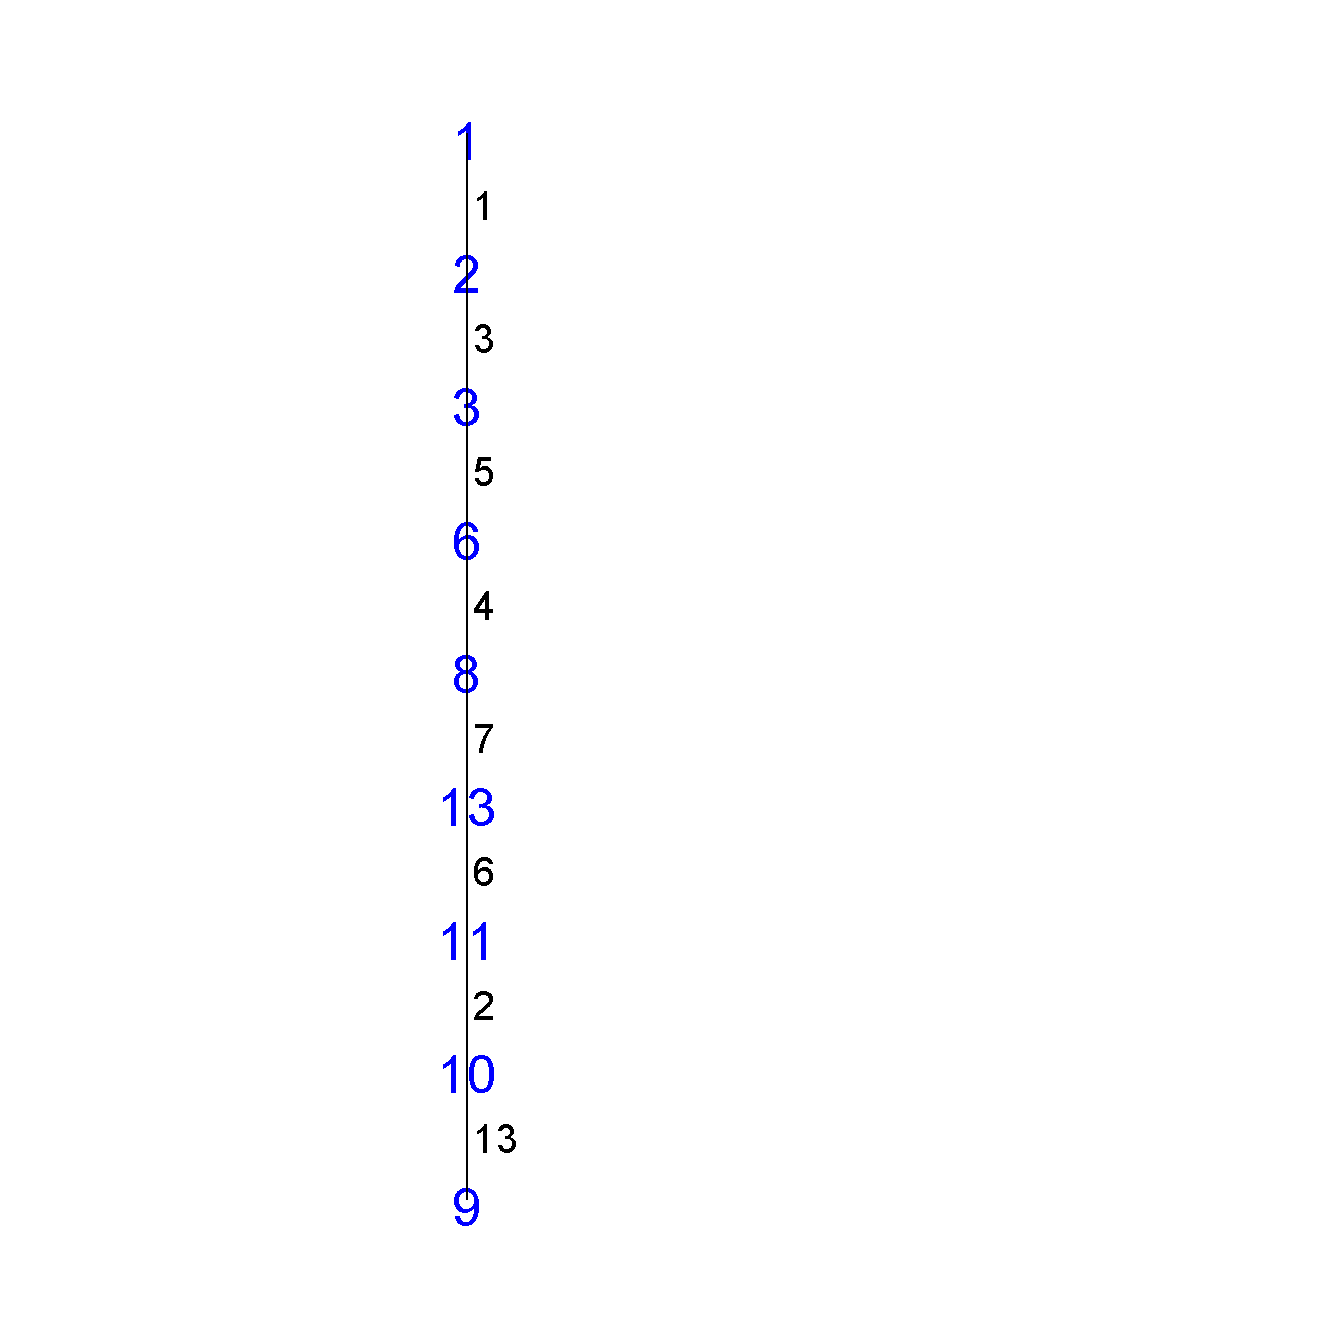
\includegraphics[width=6cm]{../sendmore/FULL/tree_expanded_9}}
\only<7>{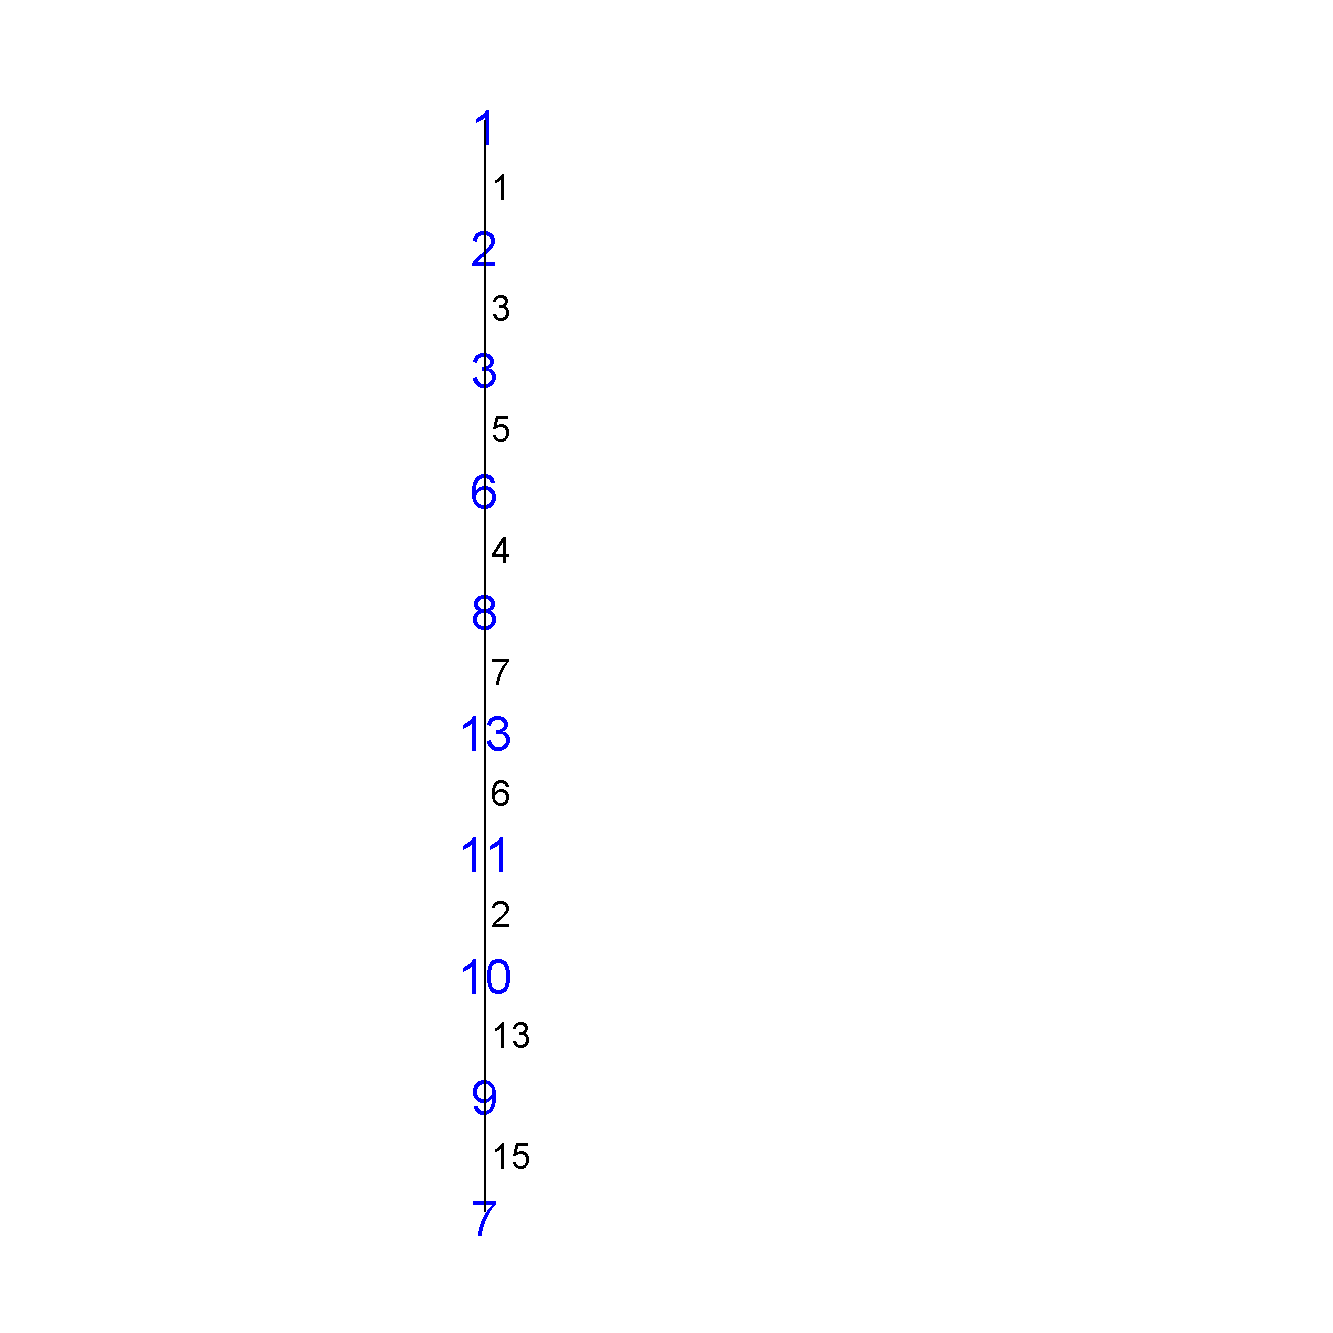
\includegraphics[width=6cm]{../sendmore/FULL/tree_expanded_10}}
\end{frame}

\begin{frame}<presentation>
\frametitle{Complete Search Tree}
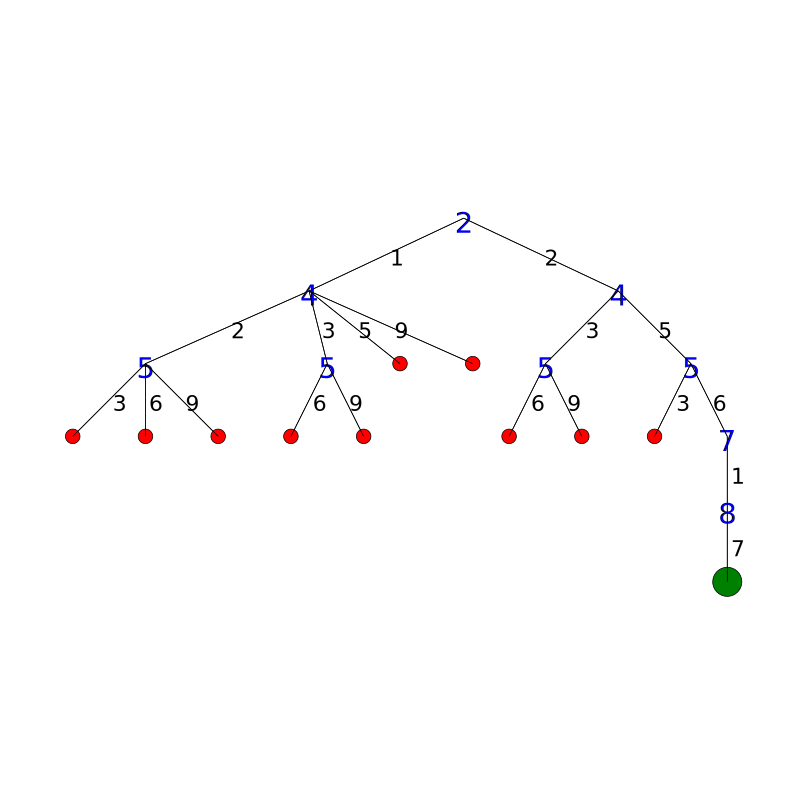
\includegraphics[width=6cm]{../sendmore/FULL/tree_expanded}
\end{frame}

\begin{figure}[ht]
\caption{\label{sendmore:First Solution} Complete Search Tree}
\begin{center}
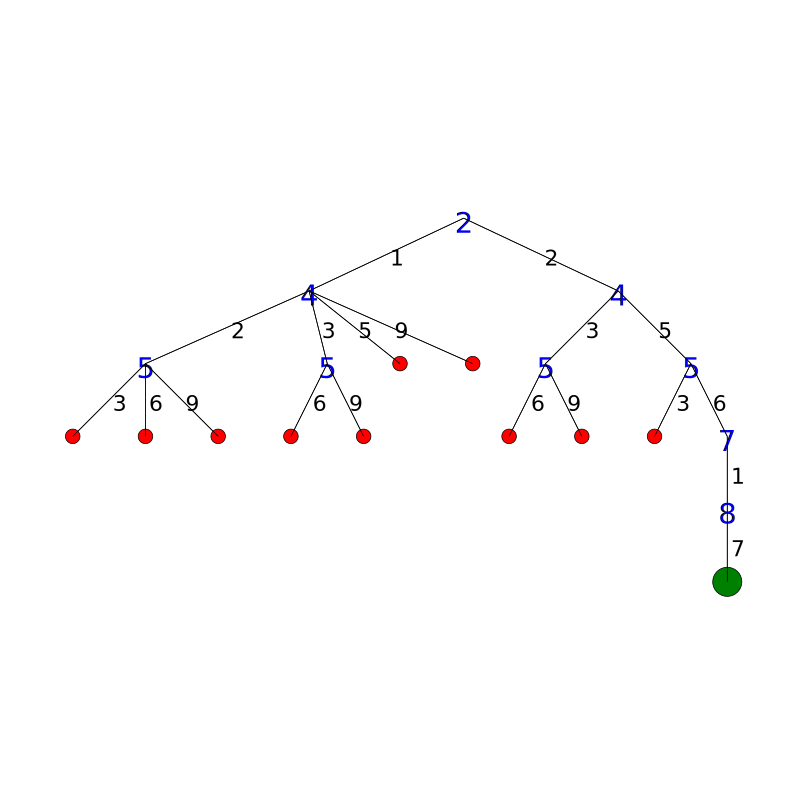
\includegraphics[width=10cm]{../sendmore/FULL/tree_expanded}
\end{center}
\end{figure}

\begin{frame}
  \frametitle{Search Tree with Gecode/GIST}
  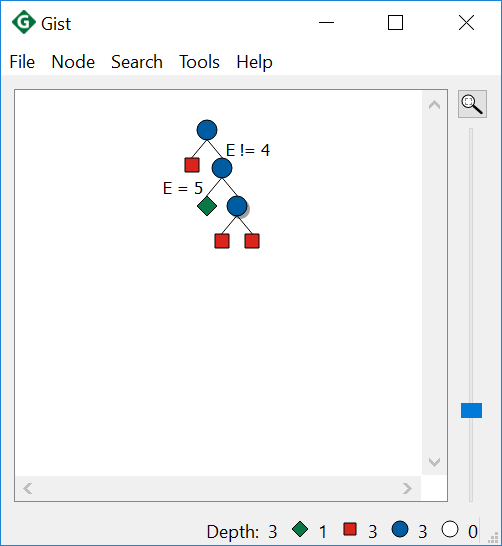
\includegraphics[width=6.5cm]{../sendmore/images/gisttree}
\end{frame}

\begin{frame}
  \frametitle{Some Differences}
  \begin{itemize}
  \item Uses binary branching 
  \begin{itemize}
  \item var equal value, var not equal value
  \end{itemize}
  \item Solutions in green, failure leafs in red, internal nodes in blue
  \item By default, shows all failed sub trees collapsed
  \item By default, uses different search strategy
  \end{itemize}
\end{frame}



All variables have been assigned, the search succeeds. Figure~\ref{sendmore:First Solution} shows the resulting search tree. There is only a single variable ($E$) for which an actual choice had to be made, all other variables are assigned by constraint propagation. The last node at the bottom of the tree is a green success node, indicating that a solution was found.


\subsection{Solution}

\begin{frame}<presentation>
\frametitle{Solution}
\begin{center}
\begin{tabular}{rrrrr}
& 9 & 5 & 6 & 7 \\
+ & 1 & 0 & 8 & 5 \\ \hline
1 & 0 & 6 & 5 & 2
\end{tabular}

\end{center} 
\end{frame}

\begin{figure}[ht]
\caption{\label{sendmore:solution}Solution}
\begin{center}
\begin{tabular}{rrrrr}
& 9 & 5 & 6 & 7 \\
+ & 1 & 0 & 8 & 5 \\ \hline
1 & 0 & 6 & 5 & 2
\end{tabular}

\end{center}
\end{figure}


We finally reached a solution (Figure~\ref{sendmore:solution}), it is easy to check that this indeed solves the puzzle.

\clearpage
\section{Points to Remember}

\begin{frame}
\frametitle{Points to Remember}
\begin{itemize}
\item Constraint models are expressed by variables and constraints.
\item Problems can have many different models, which can behave quite differently. Choosing the best model is an art.
\item Constraints can take many different forms.
\item Propagation deals with the interaction of variables and constraints.
\item It removes some values that are inconsistent with a constraint from the domain of a variable.
\item Constraints only communicate via shared variables.
\end{itemize}
\end{frame}


\begin{frame}
\frametitle{Points to Remember}
\begin{itemize}
\item Propagation usually is not sufficient, search may be required to find a solution.
\item Propagation is data driven, and can be quite complex even for small examples.
\item The default search uses chronological depth-first backtracking, systematically exploring the complete search space.
\item The search choices and propagation are interleaved, after every choice some more propagation may further reduce the problem.
\end{itemize}
\end{frame}

\begin{frame}
\frametitle{For Puzzle Purists Only}
\begin{itemize}
\item We did not follow the puzzler ethos!
\item We should solve the puzzle without making choices
\item Even a case analysis should be avoided
\item The puzzle has a single solution, we should be able to deduce the solution
\item In the process shown, we are limited by the underlying assumptions
\begin{itemize}
\item Treat each constraint on its own, they interact only by domains of variables
\item We only use the constraints that we stated in the model
\end{itemize}
\item Can we do better than that?
\end{itemize}
\hyperlink{sendmore:not an expert}{\beamergotobutton{Skip}}
\end{frame}

\begin{frame}
\frametitle{Better Reasoning}
\begin{itemize}
\item Three possible approaches (possibly many more)
\begin{itemize}
\item Full domain reasoning for arithmetic, not just bound reasoning
\item Interaction of {\em sum} and {\em alldifferent} constraints
\item Deduced implied constraint
\end{itemize}
\end{itemize}
\end{frame}

\begin{frame}
\frametitle{Looking at more than just bounds}
\begin{itemize}
\item We only considered the smallest and largest values that can be achieved in the sum constraint
\item We can do more
\begin{itemize}
\item Can any of the values between be expressed as the sum of the terms
\item Consider holes in the domains, and in the range of possible values for LHS and RHS
\end{itemize}
\item Usually not done in actual solvers for arithmetic constraints
\item Easy to do with Dynamic Programming
\end{itemize}
\end{frame}

\begin{frame}
\frametitle{Consider the interaction of multiple constraints}
\begin{itemize}
\item Usually ignored, as only interaction is via domains of shared variables
\item Here: Sum and {\em alldifferent} interact
\begin{itemize}
\item When considering the bounds, we cannot assume that each variable takes its smallest/largest value independently
\item Find feasible assignment that minimizes/maximizes the total weight
\item To do this properly, we need some non-trivial reasoning
\end{itemize}
\item Do we do this combined reasoning automatically, or only when prompted by the modeler?
\end{itemize}
\end{frame}

\begin{frame}[fragile]
\frametitle{Deduced Implied Constraints}
\begin{itemize}
\item Look at the partially solved puzzle
\item \texttt{\shortstack[r]{9END\\+10RE\\-----\\10NEY}}
\item In the hundreds position, we have $E+0+C_{10}=N+10*C_{100}$, with $C_{10}$ the 0/1 carry from the tens position
\item NB: No carry $C_{100}$ into the thousands, $C_{100}=0$
\item N must be equal to  $E+1$ with $C_{10}=1$
\item If $C_{10}=0$, then $N=E$, not possible
\item We can substitute $N=E+1$ into our main equation, but keep $N=E+1$ as well
\end{itemize}
\end{frame}

\begin{frame}
\frametitle{Expert Mode Reasoning}
\only<1>{
Starting with
\[
91*E^{4..7}+10*R^{2..8}+D^{2..8} = 90*N^{5..8}+Y^{2..8}
\]
}
\only<2>{
we get
\[
91*E^{4..7}+10*R^{2..8}+D^{2..8} = 90*E^{4..7}+90+Y^{2..8}
\]
}
\only<3>{
Eliminating duplicate occurrences of E
\[
\underbrace{E^{4..7}+10*R^{2..8}+D^{2..8}}_{26..95} = \underbrace{90+Y^{2..8}}_{92..98}
\]
shared range 92..95
}
\only<4>{
To reach 92, R must be equal to 8, therefore N, E, D, Y must be less than 8

As $N=E+1$, E must be less than 7
\[
E^{4..6}+10*8+D^{2..7} = 90+Y^{2..7}
\]
}
\only<5>{
Simplification yields
\[
\underbrace{E^{4..6}+D^{2..7}}_{6..13} = \underbrace{10+Y^{2..7}}_{12..17}
\]
shared range 12..13
}
\only<6>{
To reach 12 on LHS, E must be greater than 4, D must be greater than 5

To reach 13 in RHS, Y must be smaller than 4 
\[
E^{5..6}+D^{6..7} = 10+Y^{2..3}
\]
}
\only<7>{
As both N and D must be in 6..7, no other variable can use those values

NB: This requires better reasoning than {\em forward checking} on the {\em alldifferent} constraint

If we remove 6 from the domain of E, E must be $E=5$, and thus $N = 6$, due to $N=E+1$

{\em Alldifferent} forces $D=7$, leaving
\[
5+7 = 10+Y^{2..4}
\]
}
\only<8>{
This only leaves $Y =2$ 
\[
5+7 = 10+2
\]
That is a solution, the constraint is satisfied
}
\end{frame}


\begin{frame}
\frametitle{Expert Mode Summary}
\begin{itemize}
\item Often there is more propagation that can be done
\item Can be difficult/expensive to do
\item Balancing 
\begin{itemize}
\item How much work it done at each step of search?
\item How many steps of search you need?
\end{itemize}
\item For hard problems, doing all possible propagation may be exponential
\item Not aware that any CP system does the full reasoning shown here
\end{itemize}
\end{frame}


\begin{frame}
\frametitle{This is how people solve the puzzle by hand}
\label{sendmore:not an expert}
\href{https://www.youtube.com/watch?v=zLUCWsEeEg8}{
\includegraphics[width=8cm]{../sendmore/maxmathgames}}

\begin{itemize}
\item When writing the first version of this puzzle for CHIP (in 1986), we wanted to mimic the way we solve the puzzle by hand
\end{itemize}

\end{frame}




